\documentclass[12pt, a4paper,
%oneside,      %% -- odkomentujte, pokud chcete svou práci mít pouze jednostrannou, mezera pro hřbet pak automaticky bude pouze na levé straně
%twoside,        %% -- pro oboustranné práce, mezera pro hřbet následně střídá strany.
openright
]{report}

%% Nutné balíčky a nastavení
%%%%%%%%%%%%%%%%%%%%%%%%%%%%

%% Proměnné
\newcommand\obor{INFORMAČNÍ TECHNOLOGIE} %% -- napiš číslo a název tvého oboru
\newcommand\kodOboru{18-20-M/01} %% -- napiš číslo a název tvého oboru
\newcommand\zamereni{se zaměřením na počítačové sítě a programování} %% -- napiš číslo a název tvého oboru
\newcommand\skola{Střední škola průmyslová a umělecká, Opava} %% vyplň název školy
\newcommand\trida{IT4} %% vyplň jméno svého konzultanta
\newcommand\jmenoAutora{Matěj Kotrba}  %% vyplň své jméno
\newcommand\skolniRok{2023/24} %% vyplň rok
\newcommand\datumOdevzdani{1. 1. 2024} %% vyplň rok
\newcommand\nazevPrace{Effio - webová aplikace pro vytváření testů} %% vyplň název své práce

\title{\nazevPrace} %% -- Název tvé práce
\author{\jmenoAutora} %% -- tvé jméno
\date{\datumOdevzdani} %% -- rok, kdy píšeš SOČku

\usepackage[top=2.5cm, bottom=2.5cm, left=3.5cm, right=1.5cm]{geometry} %% nastaví okraje, left -- vnitřní okraj, right -- vnější okraj

\usepackage[czech]{babel} %% balík babel pro sazbu v češtině
\usepackage[utf8]{inputenc} %% balíky pro kódování textu
\usepackage[T1]{fontenc}
\usepackage{cmap} %% balíček zajišťující, že vytvořené PDF bude prohledávatelné a kopírovatelné
\usepackage{indentfirst}

\usepackage{graphicx} %% balík pro vkládání obrázků

\usepackage{subcaption} %% balíček pro vkládání podobrázků

\usepackage{hyperref} %% balíček, který v PDF vytváří odkazy

\linespread{1.25} %% řádkování
\setlength{\parskip}{0.5em} %% odsazení mezi odstavci


\usepackage[pagestyles]{titlesec} %% balíček pro úpravu stylu kapitol a sekcí
\titleformat{\chapter}[block]{\scshape\bfseries\LARGE}{\thechapter}{10pt}{\vspace{0pt}}[\vspace{-22pt}]
\titleformat{\section}[block]{\scshape\bfseries\Large}{\thesection}{10pt}{\vspace{0pt}}
\titleformat{\subsection}[block]{\bfseries\large}{\thesubsection}{10pt}{\vspace{0pt}}


\usepackage{tocloft} % Balíček umožní přizpůsobit vzhled tabulky obsahu
\setlength{\cftbeforechapskip}{0pt}  % Menší rozestup pro kapitoly
\setlength{\cftbeforesecskip}{0pt}   % Menší rozestup pro sekce

\setcounter{secnumdepth}{2}
\setcounter{tocdepth}{1}
\usepackage{fancyhdr}
\pagestyle{fancy}
\renewcommand{\headrulewidth}{0.025pt}

\usepackage{booktabs}

\usepackage{url}

%% Balíčky co se můžou hodit :) 
%%%%%%%%%%%%%%%%%%%%%%%%%%%%%%%

\usepackage{pdfpages} %% Balíček umožňující vkládat stránky z PDF souborů, 

\usepackage{upgreek} %% Balíček pro sazbu stojatých řeckých písmen, třeba u jednotky mikrometr. Například stojaté mí: \upmu, stojaté pí: \uppi

\usepackage{amsmath}    %% Balíčky amsmath a amsfonts 
\usepackage{amsfonts}   %% pro sazbu matematických symbolů
\usepackage{esint}     %% pro sazbu různých integrálů (např \oiint)
\usepackage{mathrsfs}
\usepackage{helvet} % Helvet font
\usepackage{mathptmx} % Times New Roman
\usepackage{Oswald} % Oswald font
\usepackage{float}

%% makra pro sazbu matematiky
\newcommand{\dif}{\mathrm{d}} %% makro pro sazbu diferenciálu, místo toho
%% abych musel psát '\mathrm{d}' mi stačí napsat '\dif' což je mnohem 
%% kratší a mohu si tak usnadnit práci

\usepackage{listings}
\usepackage{xcolor}

\renewcommand{\lstlistingname}{Kód}% Listing -> Algorithm
\renewcommand{\lstlistlistingname}{Seznam programových kódů}% List of Listings -> List of Algorithms

%% Definice 
\lstdefinelanguage{JavaScript}{
	morekeywords=[1]{break, continue, delete, else, for, function, if, in,
		new, return, this, typeof, var, void, while, with},
	% Literals, primitive types, and reference types.
	morekeywords=[2]{false, null, true, boolean, number, undefined,
		Array, Boolean, Date, Math, Number, String, Object},
	% Built-ins.
	morekeywords=[3]{eval, parseInt, parseFloat, escape, unescape},
	sensitive,
	morecomment=[s]{/*}{*/},
	morecomment=[l]//,
	morecomment=[s]{/**}{*/}, % JavaDoc style comments
	morestring=[b]',
	morestring=[b]"
}[keywords, comments, strings]


\lstdefinelanguage[ECMAScript2015]{JavaScript}[]{JavaScript}{
	morekeywords=[1]{await, async, case, catch, class, const, default, do,
		enum, export, extends, finally, from, implements, import, instanceof,
		let, static, super, switch, throw, try},
	morestring=[b]` % Interpolation strings.
}

\lstalias[]{ES6}[ECMAScript2015]{JavaScript}

% Nastavení barev
% Requires package: color.
\definecolor{mediumgray}{rgb}{0.3, 0.4, 0.4}
\definecolor{mediumblue}{rgb}{0.0, 0.0, 0.8}
\definecolor{forestgreen}{rgb}{0.13, 0.55, 0.13}
\definecolor{darkviolet}{rgb}{0.58, 0.0, 0.83}
\definecolor{royalblue}{rgb}{0.25, 0.41, 0.88}
\definecolor{crimson}{rgb}{0.86, 0.8, 0.24}


\lstdefinestyle{JSES6Base}{
	backgroundcolor=\color{white},
	basicstyle=\ttfamily,
	breakatwhitespace=false,
	breaklines=false,
	captionpos=b,
	columns=fullflexible,
	commentstyle=\color{mediumgray}\upshape,
	emph={},
	emphstyle=\color{crimson},
	extendedchars=true,  % requires inputenc
	fontadjust=true,
	frame=single,
	identifierstyle=\color{black},
	keepspaces=true,
	keywordstyle=\color{mediumblue},
	keywordstyle={[2]\color{darkviolet}},
	keywordstyle={[3]\color{royalblue}},
 literate=%
{á}{{\'a}}1 {č}{{\v{c}}}1 {ď}{{\v{d}}}1 {é}{{\'e}}1 {ě}{{\v{e}}}1
{í}{{\'i}}1 {ň}{{\v{n}}}1 {ó}{{\'o}}1 {ř}{{\v{r}}}1 {š}{{\v{s}}}1
{ť}{{\v{t}}}1 {ú}{{\'u}}1 {ů}{{\r{u}}}1 {ý}{{\'y}}1 {ž}{{\v{z}}}1,		
	numbers=left,
	numbersep=5pt,
	numberstyle=\tiny\color{black},
	rulecolor=\color{black},
	showlines=true,
	showspaces=false,
	showstringspaces=false,
	showtabs=false,
	stringstyle=\color{forestgreen},
	tabsize=2,
	title=\lstname,
	upquote=true  % requires textcomp
}

\lstdefinestyle{JavaScript}{
	language=JavaScript,
	style=JSES6Base,
}
\lstdefinestyle{ES6}{
	language=ES6,
	style=JSES6Base
}

\usepackage{lipsum} %% balíček který píše lipsum (nesmyslný text, který se používá pro kontrolu typografie)

%% Začátek dokumentu
%%%%%%%%%%%%%%%%%%%%
\begin{document}
	
	\pagestyle{empty}
	\pagenumbering{Roman}
	
	\cleardoublepage

%% Titulní stránka s informacemi
%%%%%%%%%%%%%%%%%%%%%%%%%%%%%%%%%%%%%%%%
	
	{\fontfamily{phv}\selectfont
		%% Logo školy
		\begin{figure}[h]
			\centering
			
\includegraphics[width=0.6\linewidth]{image/logo-skoly.png} 
		\end{figure}
		
		
		%% Hlavička práce a její název (viz proměnná \nazev prace)
		%% \sffamily %%% bezpatkové písmo - sans serif
		{\bfseries %%% písmo na stránce je tučně
			\begin{center}
				\vspace{0.025 \textheight}
				\LARGE{ZÁVĚREČNÁ STUDIJNÍ PRÁCE}\\
				\large{dokumentace}\\
				\vspace{0.075 \textheight}
				\LARGE {\nazevPrace}\\
			\end{center}  
		}%%%
		
		\begin{figure}[h]
			\centering
			
\includegraphics[width=0.8\linewidth]{image/effio.png} 
		\end{figure}
		
		\vspace{0.02 \textheight}
		\begin{table}[h!]
			\begin{tabular}{ll}
				\textbf{Autor:} & \jmenoAutora\\ 
				\textbf{Obor:} & \kodOboru { } \obor\\
				\textbf{} & \zamereni\\
				\textbf{Třída:} & \trida\\
				\textbf{Školní rok:} & \skolniRok\\
			\end{tabular}
			
		\end{table}		
	}
	
\cleardoublepage %% Zalomení dvojstránky
	
%% Stránka obsahující poděkování a prohlášení
%%%%%%%%%%%%%%%%%%%%%%%%%%%%%%%%%%%%%%%%%%%%%%%%%%%%%%%%

%% Poděkování - nepovinné
%%%%%%%%%%%%%%%%%%%%%%%%%%%%
	
	\noindent{\large{\bfseries{Poděkování}\\}}
	\noindent Rád bych poděkoval Mgr. Markovi Lučnému za poskytuntí konzultace ohledně tohoto projektu.
	
	\vspace*{0.7\textheight} %% Vertikální mezeru je možné upravit

%% Prohlášení - povinné
%%%%%%%%%%%%%%%%%%%%%%%%%%%%
	\noindent{\large{\bfseries{Prohlášení}\\}}  %% uprav si koncovky podle toho na jaký rod se cítíš, vypadá to pak lépe :) 
	\noindent{Prohlašuji, že jsem závěrečnou práci vypracoval samostatně a uvedl veškeré použité 
		informační zdroje.\\}
	\noindent{Souhlasím, aby tato studijní práce byla použita k výukovým a prezentačním účelům na Střední průmyslové a umělecké škole v Opavě, Praskova 399/8.}
	\vfill
	\noindent{V Opavě \datumOdevzdani\\}
	\noindent
	\begin{minipage}{\linewidth}
		\hspace{9.5cm} 
		\begin{tabular}{@{}p{6cm}@{}}
			\dotfill \\
			Podpis autora
		\end{tabular}
	\end{minipage}
	
	\cleardoublepage %% Zalomení dvojstránky

%% Stránka obsahující abstrakt (anotaci)
%%%%%%%%%%%%%%%%%%%%%%%%%%%%%%%%%%%%%%%%%%%%%%%%%%%%%%%%	

%% Abstrakt v češtině
%%%%%%%%%%%%%%%%%%%%%%%%%%%%
	\noindent{\Large{\bfseries{Anotace}\\}}
	\noindent Výsledkem projektu je funkční webová aplikace pro vytváření a vyplňování testů, které se skládají z~různých možností otázek včetně programovací. Aplikace zahrnuje přihlášení přes Google a GitHub. Uživatel vytváří jednotlivé testy výběrem šablony, nebo importem z GIFT formátu, otázek, komentářů a následně upravuje detaily testu jako jméno, popis, obrázek, upravitelný známkovací systém, zařazení do skupin a tagy. Hotový test může sám zkusit z~vlastní kolekce testů a nebo z~komunitního centra, kde se nacházejí komunitou vytvořené testy, po vyplnění testu se uživateli objeví výsledky a známka. Krom výroby a vyplňování testů aplikace obsahuje také skupiny, kde mohou mezi sebou uživatelé komunikovat pomocí chatu a majitel do ní může sdílet testy, na dříve vyplněné testy se může podívat v sekci testové historie. Přehled o aktivitě uživatele si může prohlédnout v dashboardu prostřednictvím vizuálních grafů. Dříve vytvořené testy se dají v části kolekce editovat, mazat a také exportovat do GIFT formátu v textovém souboru pro použití například v~Moodlu. Aplikace disponuje zcela responsivním designem se světlým a tmavým režimem.
	
	\vspace{18pt}
	
	\noindent{\large{\bfseries{Klíčová slova}}}
	
	\noindent webová aplikace, databáze, responsivní design, účty, grafy, tvorba testů, barevné režimy
	
	\vspace{18pt}


	
	\clearpage %% Zalomení stránky

%% Stránka s generovaným obsahem
%%%%%%%%%%%%%%%%%%%%%%%%%%%%%%%%%%%%%%%	
	
	\tableofcontents %% Vygeneruje tabulku s obsahem

	\pagenumbering{arabic} %% Nastavení způsobu číslování stránek (alternativy roman | Roman)
	\setcounter{page}{1} %% Nastavení počitadla stránek

%% Stránka s úvodem - povinná část
%%%%%%%%%%%%%%%%%%%%%%%%%%%%%%%%%%%%%%%		
	\chapter*{Úvod}
	\label{intro}
%Tento příkaz vytvoří novou kapitolu s názvem "Úvod" ve vašem dokumentu.
%Hvězdička * u příkazu \chapter* znamená, že tato kapitola nebude mít číslo. Ve výsledném dokumentu se tedy objeví jako "Úvod" bez předcházejícího čísla kapitoly, které se obvykle zobrazuje u číslovaných kapitol.
%Tento příkaz také znamená, že kapitola se automaticky neobjeví v obsahu, protože LaTeX standardně zahrnuje do obsahu pouze číslované kapitoly.
	\addcontentsline{toc}{chapter}{Úvod}
%Tento příkaz ručně přidává záznam do obsahu.
%První parametr toc označuje, že přidáváme záznam do Table of Contents (obsahu).
%Druhý parametr chapter specifikuje úroveň záznamu. V tomto případě říkáme, že přidávaný záznam má být považován za kapitolu.
%Třetí parametr Úvod je text, který se objeví v obsahu. V tomto případě bude v obsahu zobrazen název "Úvod".	
V dnešní době se běžně využívají webové aplikace, které umožňují vytváření testů/kvízů, které poté jiní uživatelé vyplňují. Prostředí těchto aplikací jsou však často nepřehledné a vytváření testů či kvízů je úporné. S touto myšlenkou jsem se rozhodl vytvořit aplikaci, která by kombinovala možnosti jiných aplikací s přehledným moderním zobrazením a dalšími užitečnými prvky.

Má aplikace by krom již zmíněné funkcionality pro tvorbu testů a kvízů měla do jisté míry umožňovat prvky sociálních sítí jako třeba skupiny, komunitní místo kde by se mimo jiné zobrazovaly testy ostatních uživatelů. Hlavní myšlenkou bylo vytvořit nejen aplikaci jako takovou ale také využít moderní technologie a postupy, neboli vytvořit ji \uv{typesafe}, bez potřeby vlastního serveru za pomocí cloudové technologie \uv{serverless} a plně responzivní pro uživatele na kterémkoli zařízení.

V dokumentaci jsou popsané využité technologie, postupy a jednotlivé funkcionality celé aplikace. První část popisuje architekturu a přístup k~řešení, ve druhé části popisuji využité technologie a jejich účel v~aplikaci, ve třetí části se potom zmiňuji o různých možnostech, které Effio nabízí. Nakonec se poohlížím na dosažené cíle a možné vylepšení.

%Tipy k psaní úvodu
%Je povinný, nadpis neměňte, rozsah - max. 1 strana. 
%Tato část práce obsahuje: 
%* náhled do řešené problematiky, zdůvodnění volby problematiky, 
%* předem definované cíle práce, 
%* motivaci pro další čtení textu včetně stručného uvedení obsahu následujících kapitol 


\chapter{Architektura a koncepty aplikace}

\section{Architektura}

Vzhledem k tomu, že záměrem bylo vytvořit aplikaci, která bude pro veškeré \uv{backendové} úlohy využívat cloud, tak je architektura relativně složité téma, proto se pokusím stručně popsat základní proces vykreslení stránky. Uživatel získává statické soubory ze \uv{CDN}, dynamicky vytvořené stránky pro první zobrazení (\uv{first render}) jsou generovány na instancích \uv{serverless funkcí} třetí strany, každá instance se vytváří podle potřeby na reálném serveru poskytovatele, není dedikovaná a ani nezůstavá aktivní po delší dobu. Server je dále využíván pro potřeby klienta, které si on sám nemůže obstarat především z bezpečnostních důvodů (DB queries, secret env variables...). Databáze vytváří spojení se serverem a ten získává potřebná data, viz. obrázek dole \ref{fig:effio-architecture}.
\begin{figure}[h!]
	\centering %% příkaz, který ti obrázek zarovná na střed
	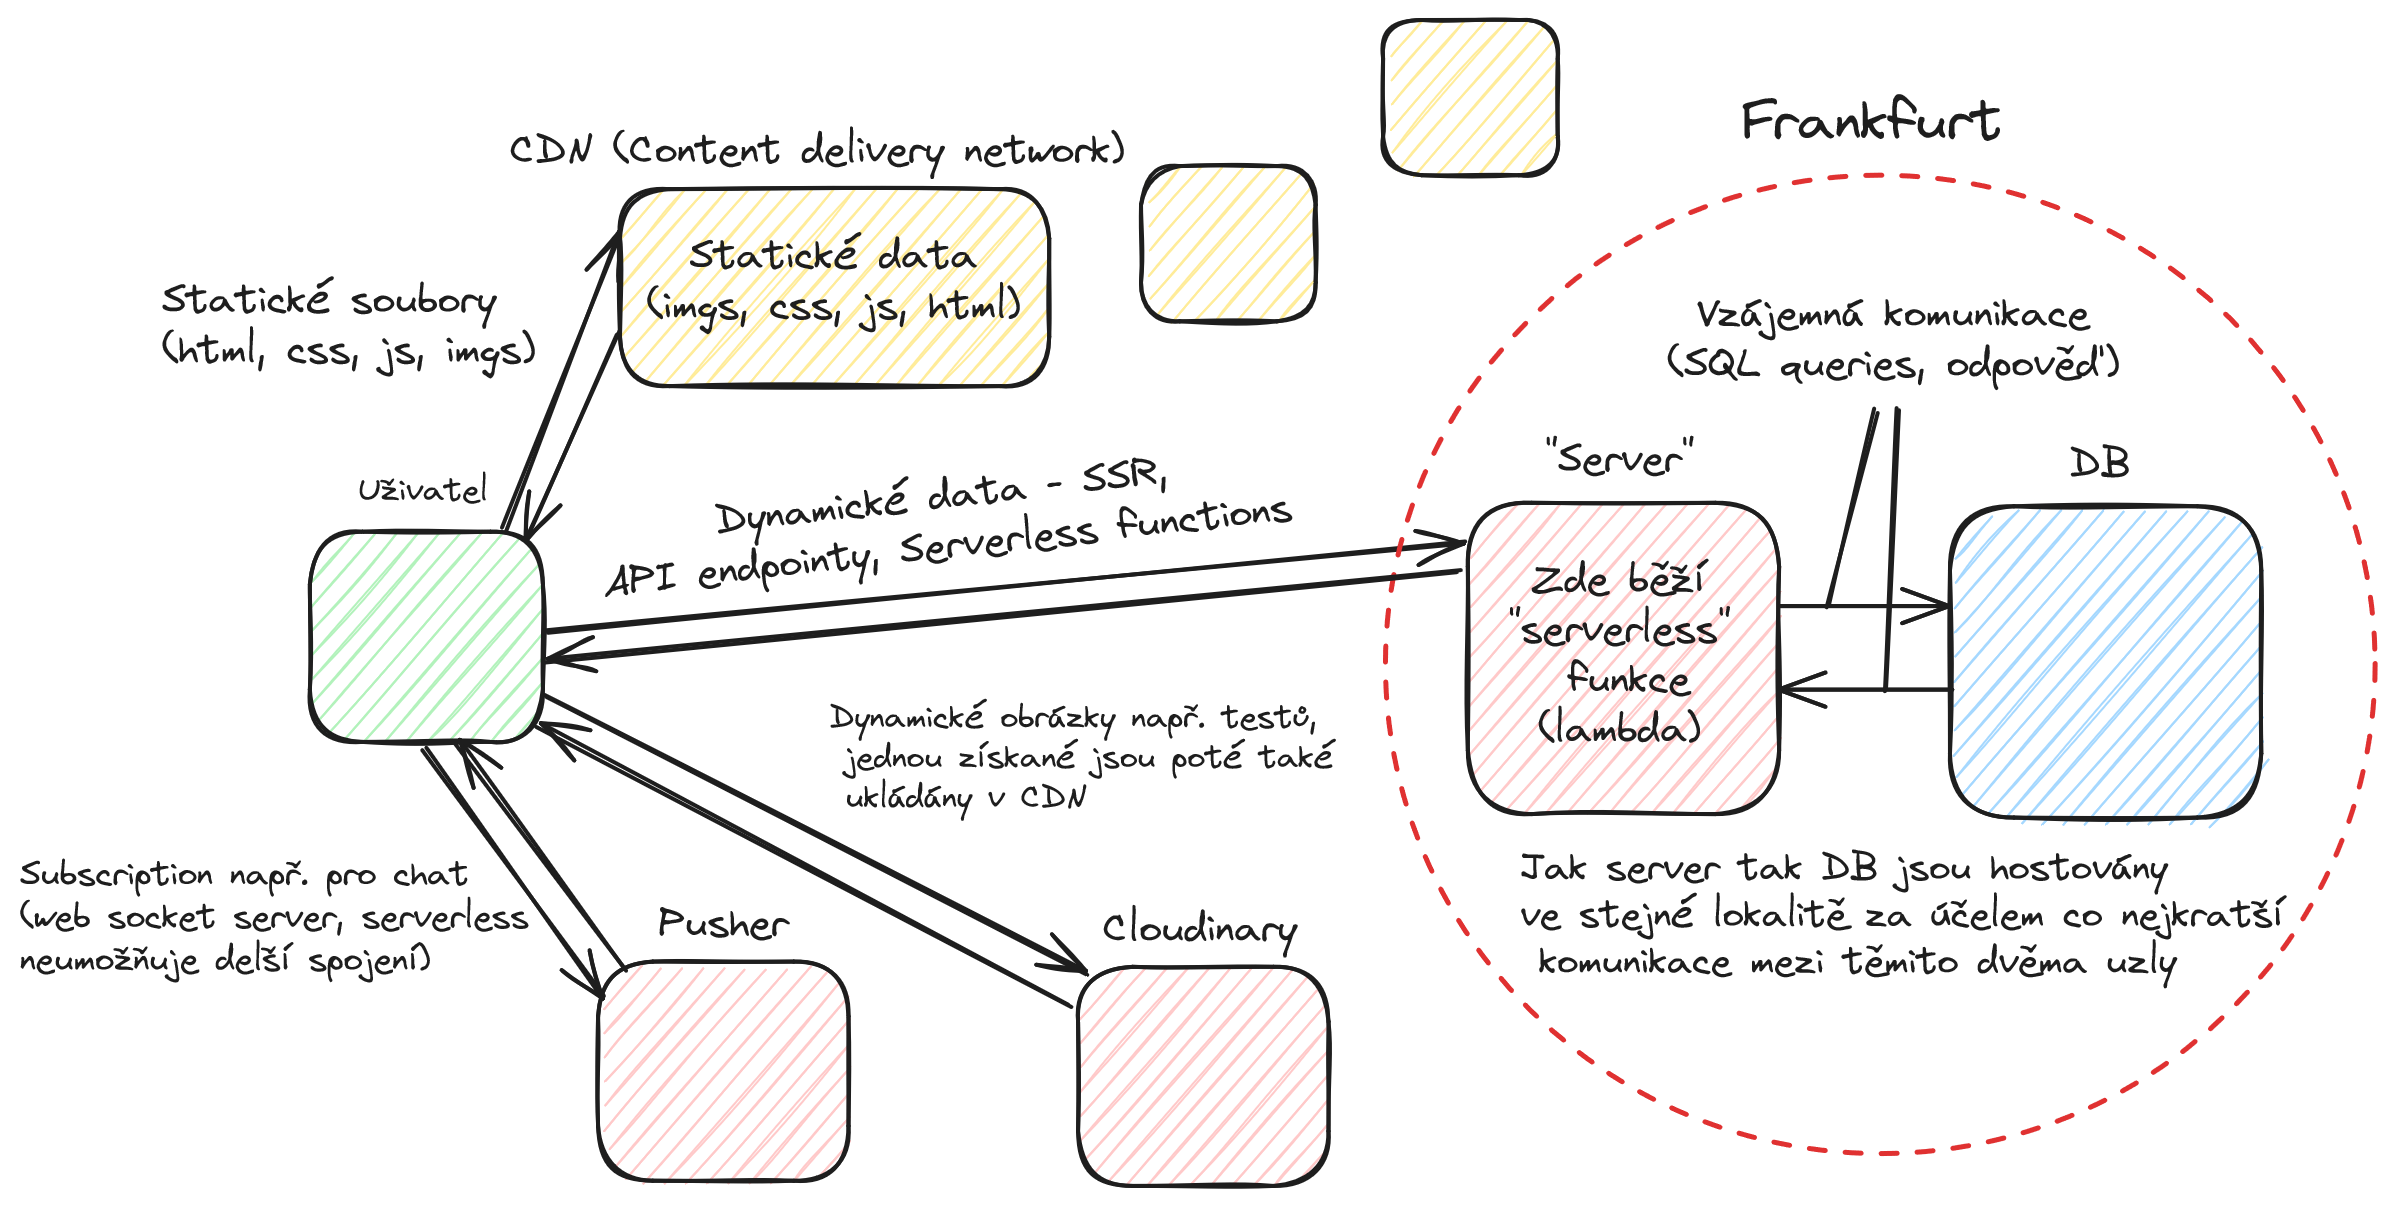
\includegraphics[width=1\linewidth]{image/effio-architecture-simple.png} 
	\caption{Jednoduchý přehled architektury Effia.} %% popisek obrázku, nezapomeň na citace!
	\label{fig:effio-architecture} %% označení až budeš chtít na obrázek odkazovat
\end{figure}

\subsection{Koncept \uv{single page application} a tradičního web serveru }
V minulé sekci jsem zmínil pojem web server, ten generuje stránku, která je poslána uživateli, ta se poté generuje znovu vždy když je uživatel přesměrován na jinout stránku, tento koncept má spoustu nevýhod jako například nemožnost jednoduše uchovávat data mezi těmito přechody.\uv{Single page application} je vlastně JavaScript framework, který se o překreslování obrazu a přesměrování stará sám za pomocí JavaScriptu bez nutnosti dotazovat se serveru o novou stránku či data. Tento přístup bohužel také není perfektní, nutnost stahovat veškerý kód nebo velice chabý SEO rating.

\subsection{Metaframework}
Oba zmíněné koncepty přinášejí své výhody ale s ním také nevýhody, Metaframework je technologie, která kombinuje výhody obou konceptů a přináší za mě nejlepší variantu jak vytvářet webovout aplikaci. Disponuje možností běhu kódu na serveru, přesměrováním na klientské části a dalšími výhodami. Takových technologií existuje celá řada, jako například populární NextJS, já si pro svůj projekt zvolil SvelteKit.

\subsection{Cloud hosting}
Jak již bylo zmíněno v~úvodu tak tato aplikace by se měla obejít bez vlastního serveru, nejde ale jenom o databázi ale také například o ukládání obrázků nebo hostování aplikace jako takové, to je prováděno přes \uv{Cloud hostingy} jako Vercel pro hostování stránky jako takové, zároveň ale řeší i rozesílání statických dat do CDN a poskytuje serverless lambda funkce, Planetscale pro hostování mojí MySQL databáze, Cloudinary, který slouží jako \uv{bucket} pro obrázky a také jejich možnost editace přes url parametry, nebo Pusher, který slouží jako web socket server například pro chat.

\section{Typesafety}

Webové aplikace standartně využívají JavaScript, ten ale obnáší signifikantní nevýhodu v podobě nemožnosti \uv{otypovat} kód, to způsobuje obtíž orientovat se v kódu, velké množství produkčních chyb a také spoustu času stráveného pochopením dříve napsaného kódu. Pro Effio jsem se tedy rozhodl využít moderní technologie a vytvořit tak téměř plně \uv{typesafe} (otypovanou) aplikaci. TypeScript v Effiu nahrazuje JavaScript, ten do tohoto jazyka přináší typy. To ale nestačí, API endpointy, stejně jako databázové dotazy stále nemůžou být otypované a proto jsem připojil také knihovny tRPC a Prisma.


\chapter{Využité technologie}

\section{SvelteKit}

Svelte je open source JavaScriptový framework vyvíjený od roku 2016 týmem Riche Harrise, jeho hlavní výhodou je rychlost ale také intuitivita, protože jazyk se snaží vypadat jako JavaScript, zatímco rozšiřuje jeho možnosti, díky tomu se za posledních let těší rostoucí popularitě webových vývojářů. Na rozdíl od ostatních frontendových frameworků (například React, Angular, Solid nebo Qwik) Svelte disponuje vlastním jazykem, který se zapisuje do \texttt{.svelte} souboru, ten se následně kompiluje do vysoce efektivního JavaScriptu.\\

SvelteKit je metaframework postavený na Svelte. Jeho hlavní výhody se skládají z:
\begin{itemize}
	\item Rychlost - Svelte vytváří velice rychlou aplikaci, v kombinaci s Vitem (bundler) se ale také spojuje s velice rychlým build timem a fast refreshy. To ale není jediné místo kde se rychlost projevuje, za pomocí SvelteKitu se aplikace vyvíjí velmi rychle díky velice malému množství \uv{boilerplate} kódu.
	\item Flexibilita - Aplikace často potřebuje různé typy vykreslování stránek, SvelteKit dovoluje jednoduše nakonfigurovat jednotlivé stránky či cesty pro specifické způsoby jako SPA, SSR, SSG nebo MPA.
	\item Přehlednost - SvelteKit využívá \uv{file based routing}, tedy cesty aplikace jsou generovány podle složek, které vývojář vytvoří, soubory se poté vždy jmenují stejně, \texttt{+page.svelte} pro stránku, \texttt{+layout.svelte} pro layout apod. Díky tomu je vždy jasné pro co specifický souboru slouží, přehlednosti také přidává, již u Sveltu zmíněná podobnost s JavaScriptem.
\end{itemize} 

\section{Typescript}
Typescript se dá považovat jako nadstavba JavaScriptu, poskytuje ale jednu výraznou výhodu - typy, díky nim je možno mnohem snadněji dohledávat chyby, vracet se k dříve napsanému kódu a celkově mnohem zlepší \uv{developer experience} při vytváření aplikace. Sám o sobě pomůže s otypováním jednotlivých částí kódu, neporadí si však například s API endpointy nebo databázovými dotazy, které se poté musí otypovat ručně, což je ale velice špatný způsob.

\section{tRPC}
V minulé sekci jsem se zmínil o problémech s otypováním API endpointů, tRPC (Typescript Remote Procedure Call) tento problém řeší tím, že vytváří dynamické typy pro jednotlivé endpointy, podle toho jak si je sami nadefinujeme.

\section{Prisma}
Prisma slouží jako ORM (Object–relational mapping), to znamená pomocí JavaScriptu získávat data z databáze bez přímého použití jazyka SQL, Prisma se skládá z klientské části, která pomocí protokolu založeném na JSON komunikuje se serverovou částí, tam je následně uskutečněn SQL dotaz a odpověď je poslána klientovi. Také řeší již zmíněný problém s otypováním těchto dotazů, pro Prismu je totiž nutné vytvořit \texttt{schema.prisma} soubor kde se definuje model databáze, ten poté můžeme pomocí Prisma CLI nahrávat do databáze ale také vytvářet dynamické typy, které poté využijeme jak v~dotazech tak v~aplikaci pro data, která dostaneme zpět.

\section{Zod}
Zod je validační knihovna jako např. Yup. Jeho výhodou je avšak možnost využít jeho validační schémata jako typy a také samotná validace funguje jako \uv{type guard} (kontroluje a nastavuje typy u vložené proměnné). Jeho další výhodou je například jeho nízká velikost.

\section{Tailwind CSS}
Tailwind CSS je \uv{CSS utility library}, to znamená, že narozdíl od frameworků jako je třeba Bootstrap nebo Material UI neposkytuje celé předpřipravené komponenty ale připravené CSS třídy, které se aplikují na HTML elementy, jeho výhodou je naprostá kontrola nad chováním stylů, které se aplikují, přehlednost a rychlost se kterou se dá styly vytvářet.

\section{Auth.js}
Auth.js je knihovna sloužící pro autentifikaci a autorizaci, poskytuje možnost \uv{session based}, to je použito v Effiu, a JWT autentifikace. Dále knihovna podporuje OAuth s mnohými providery, v tomto projektu je využit GitHub a Google s jednoduchou možností přidat další. Výhodou knihovny je, že data si vývojář spravuje sám, neboli jsou ukládána do jeho vlastní databáze v podobě tabulek (které si také může sám upravit): Account, Session, User a Verification Token, které poskytují naprostou kontrolu nad ověřením uživatelů.

%\section{Cloud provideři}
%Effia plně spoléhá na cloudové řešení, díky nim je jednoduché zprovoznit plně funkční stránku bez jakékoliv starosti o fyzický hardware, stejně jako o škálování zdrojů podle potřeby.
%\begin{itemize}
	%\item \textbf{Vercel} se stará o hostování aplikace jako takové, distribuci statického obsahu na %CDN a jednoduše řeší znovuvytvoření stránky po změně kódu v~GitHub repozitáři. Vercel podporuje %\uvserverless\uv architekturu v~podobě tradiční lambda funkcí. Jedná se o instance dané funkce, %která se spouští na serveru, není dedikovaná ale spouští se a vypíná podle vytížení.
%	\item \textbf{Cloudinary} slouží
%\end{itemize}

\chapter{Kroky k řešení, funkcionality aplikace a implementace}
\section{Založení a konfigurace projektu}
Prvním krokem bylo založení projektu a stažení potřebných knihoven technologií, které jsem plánoval využít. Kombinace mnou vybraných technologií nebyla kompletně konvenční a proto jsem se musel v~některých případech obrátit na komunitou vytvořené adaptéry, příkladem je například knihovna \texttt{trpc-sveltekit}, která propojuje SvelteKit a tRPC, které je primárně navrženo buď jako samostatný server a nebo jako implementace do Next.js.

\clearpage
\section{Model databáze}
Dalším krokem bylo vytvořit databázový model, vystavený obrázek nezachycuje model počáteční ale ten, ke kterému postupem práce Effio dospělo přidáváním nových funkcionalit, model byl také několikrát částečně přepracován.
\begin{figure}[H]
	\centering %% příkaz, který ti obrázek zarovná na střed
	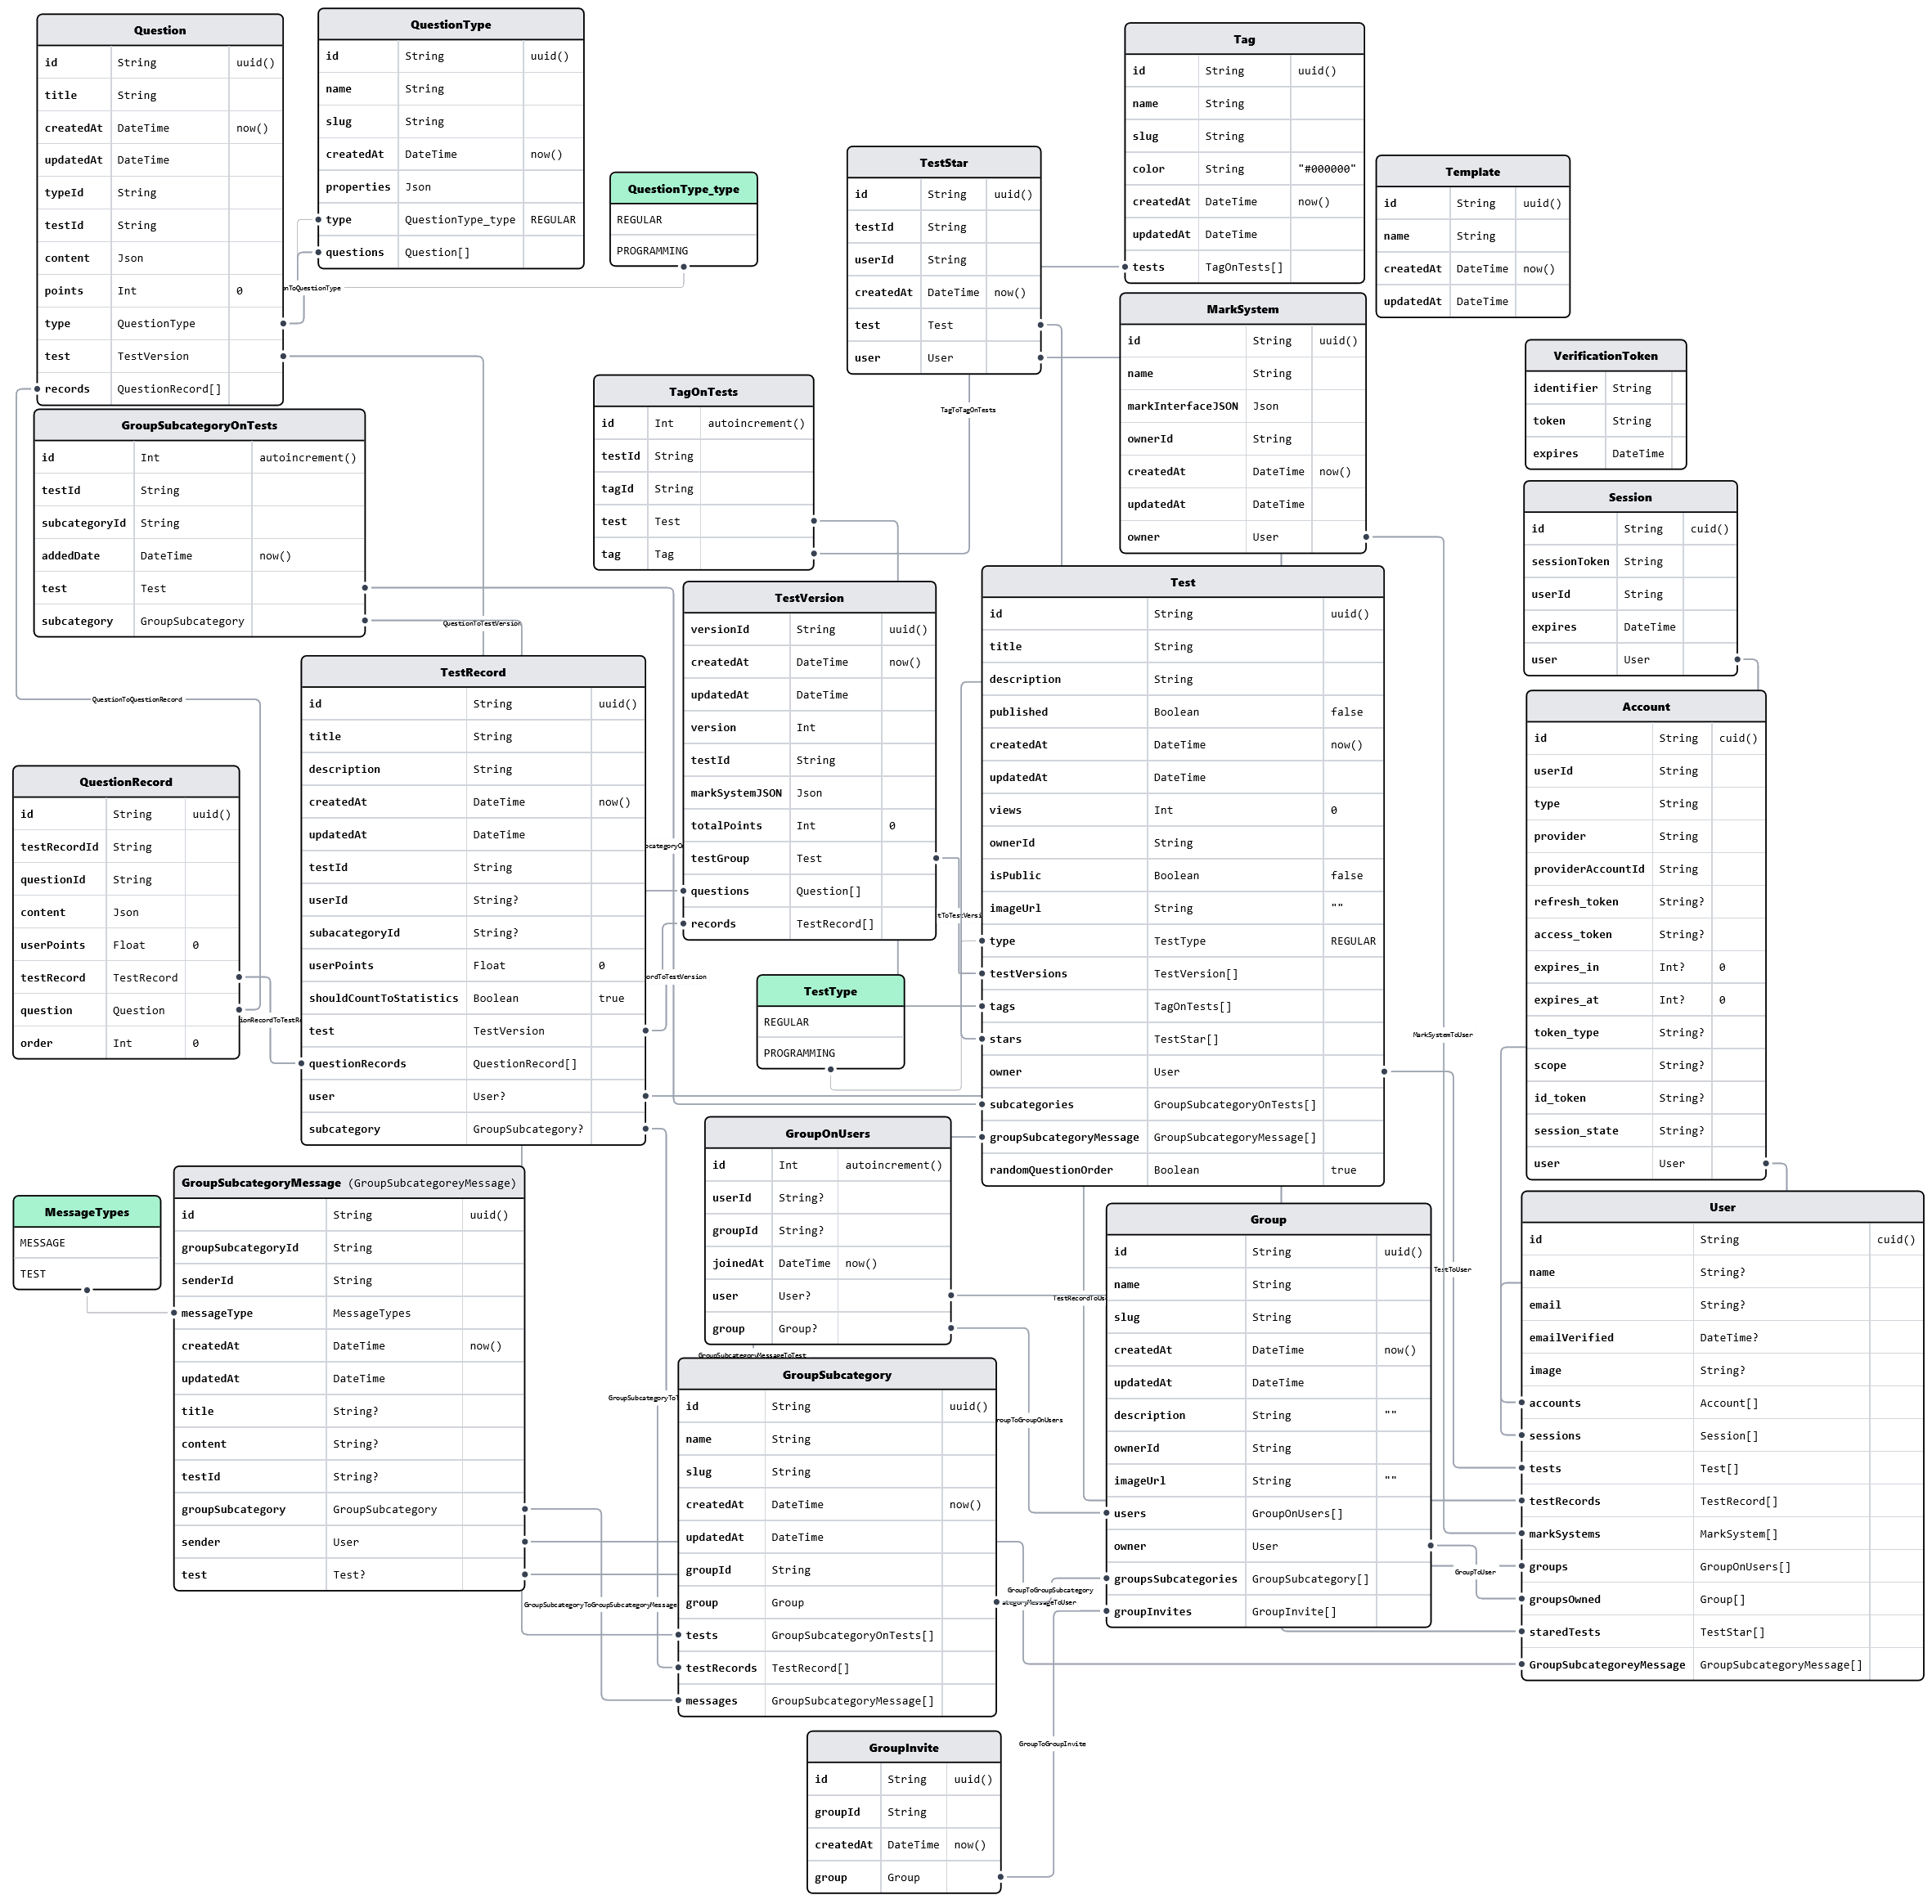
\includegraphics[width=1\linewidth]{image/schema.png} 
	\caption{Databázový model Effia. Vytvořeno pomocí \href{https://github.com/Ovyerus/prismaliser}{Prismaliser}} %% popisek obrázku, nezapomeň na citace!
	\label{fig:schema} %% označení až budeš chtít na obrázek odkazovat
\end{figure}
\clearpage
\section{Design}
Jednou z~hlavních myšlenek bylo vytvořit pohledem přívětivou aplikaci, proto se návrh designu stál klíčovou částí pro stylově propracovanější prvky stránky. Pro tvorbu designu, stejně jako vytváření a úpravu potřebných obrázků jsem využil aplikaci Figma.
\begin{figure}[h]
	\centering %% příkaz, který ti obrázek zarovná na střed
	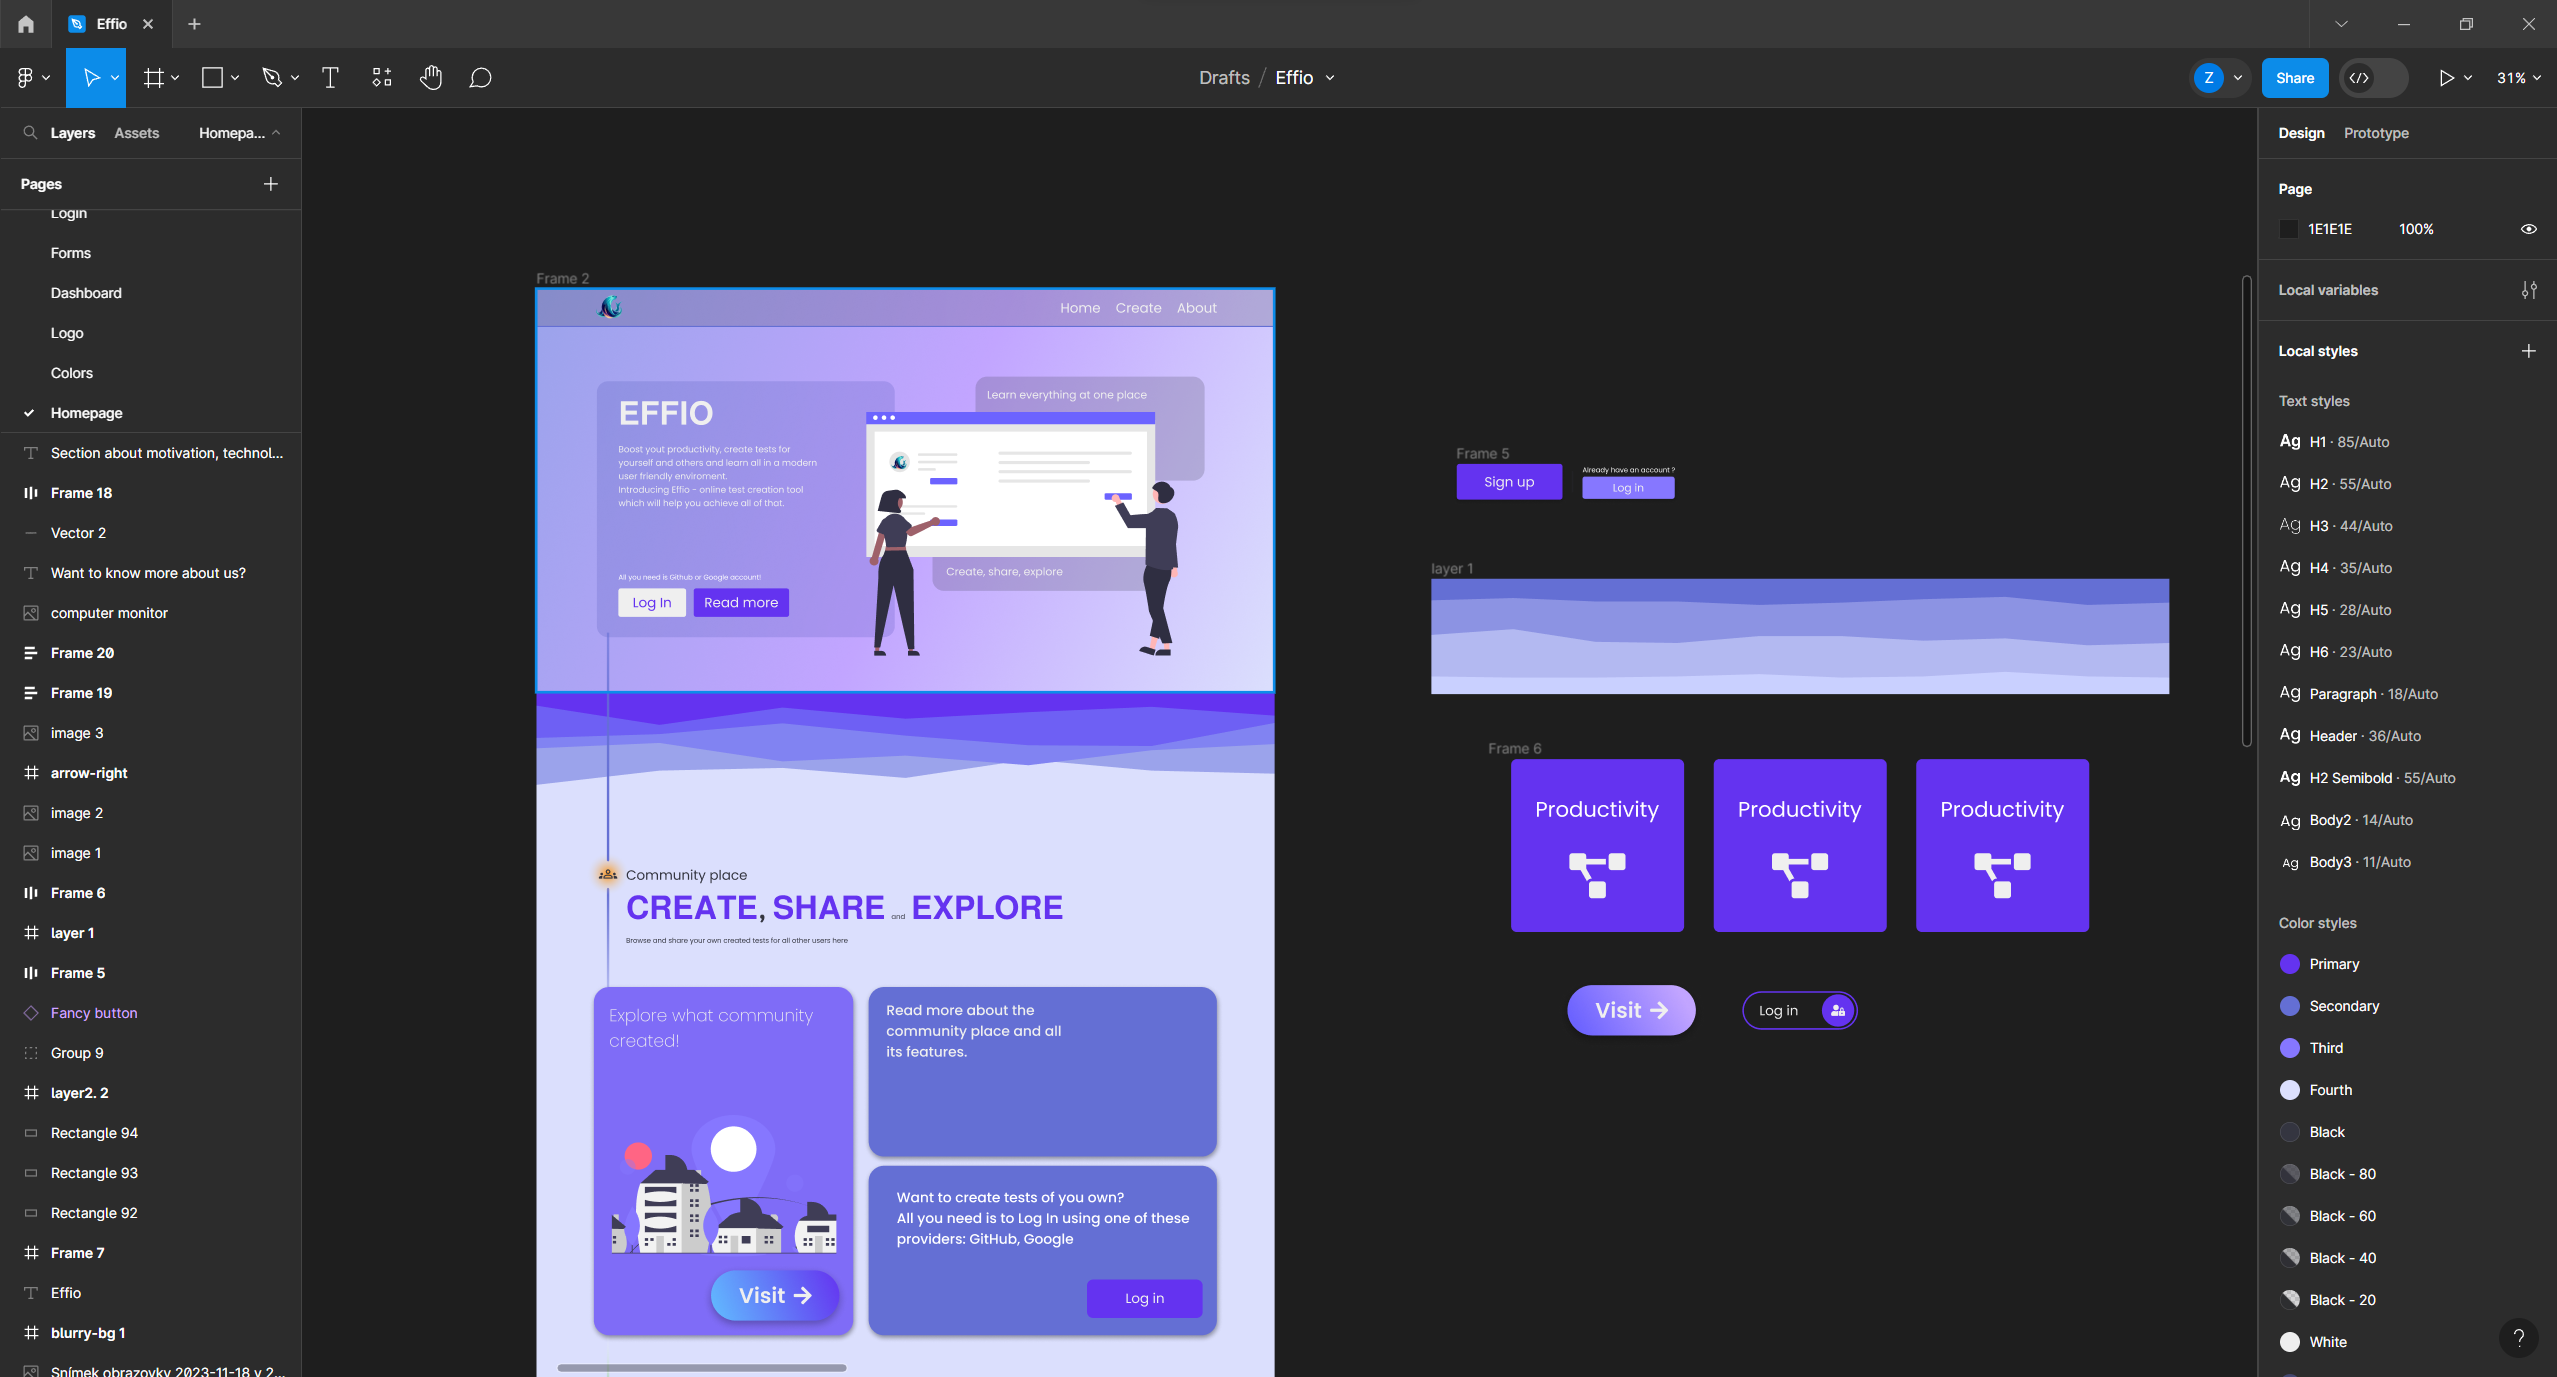
\includegraphics[width=1\linewidth]{image/figma.png} 
	\caption{Prvotní návrh domovské stránky.} %% popisek obrázku, nezapomeň na citace!
	\label{fig:figma} %% označení až budeš chtít na obrázek odkazovat
\end{figure}

\section{Testy a jejich vlastnosti}
Jednou z esenciálních funkcionalit Effia je možnost vytvořit test, k~tomuto existuje mnoho různých postupů, nad danou problematikou jsem se zprvu zamýšlel a až poté napsal funkční nástroj pro jejich vytváření ale to stejně nakonec nezabránilo následné nutnosti přepsat téměř celou funkcionalitu při vytváření testu.

\subsection{Tvorba testu}
\label{subsec:creation}
Jako první si uživatel zvolí mezi kvízovým a programovacím testem, u obou si poté vybere šablonu.
\begin{itemize}
	\item Kvízový - po výběru šablony, kde si uživatel může zvolit i import z GIFT formátu, se uživatel dostane do tvorby testu samotného, vybírat si aktuálně může z~6~typů otázek: \textit{Pick One}, \textit{True/False}, \textit{Connect}, \textit{Write}, \textit{Fill} a \textit{Geography}, otázkám lze svévolně měnit pořadí, přidávat komentáře k~odpovědím a upravovat počet získaných bodů.
	\item Programovací - po výběru šablony se uživatel dostane do tvorby testu programovacího, kde ho pojmenuje problém, popíše co má uživatel řešit, nadefinuje kontrolní vstupy a očekávané výstupy, poté může zanechat nápovědy
\end{itemize}
Po dokončení těchto úprav se uživatel dostane do konečných úprav testu, což činí jméno, popisek a obrázek testu, volitelné zařazení do skupin, tagy, rozhodne se jestli využít známkovací systém, který si může sám upravit, zvolí si zdali náhodně třídit otázky a následně tvorbu ukončí a rozhodne se zdali test uložit jako návrh nebo ho publikovat.

\begin{figure}[h]
	\centering
	\begin{minipage}[]{0.49\textwidth}
		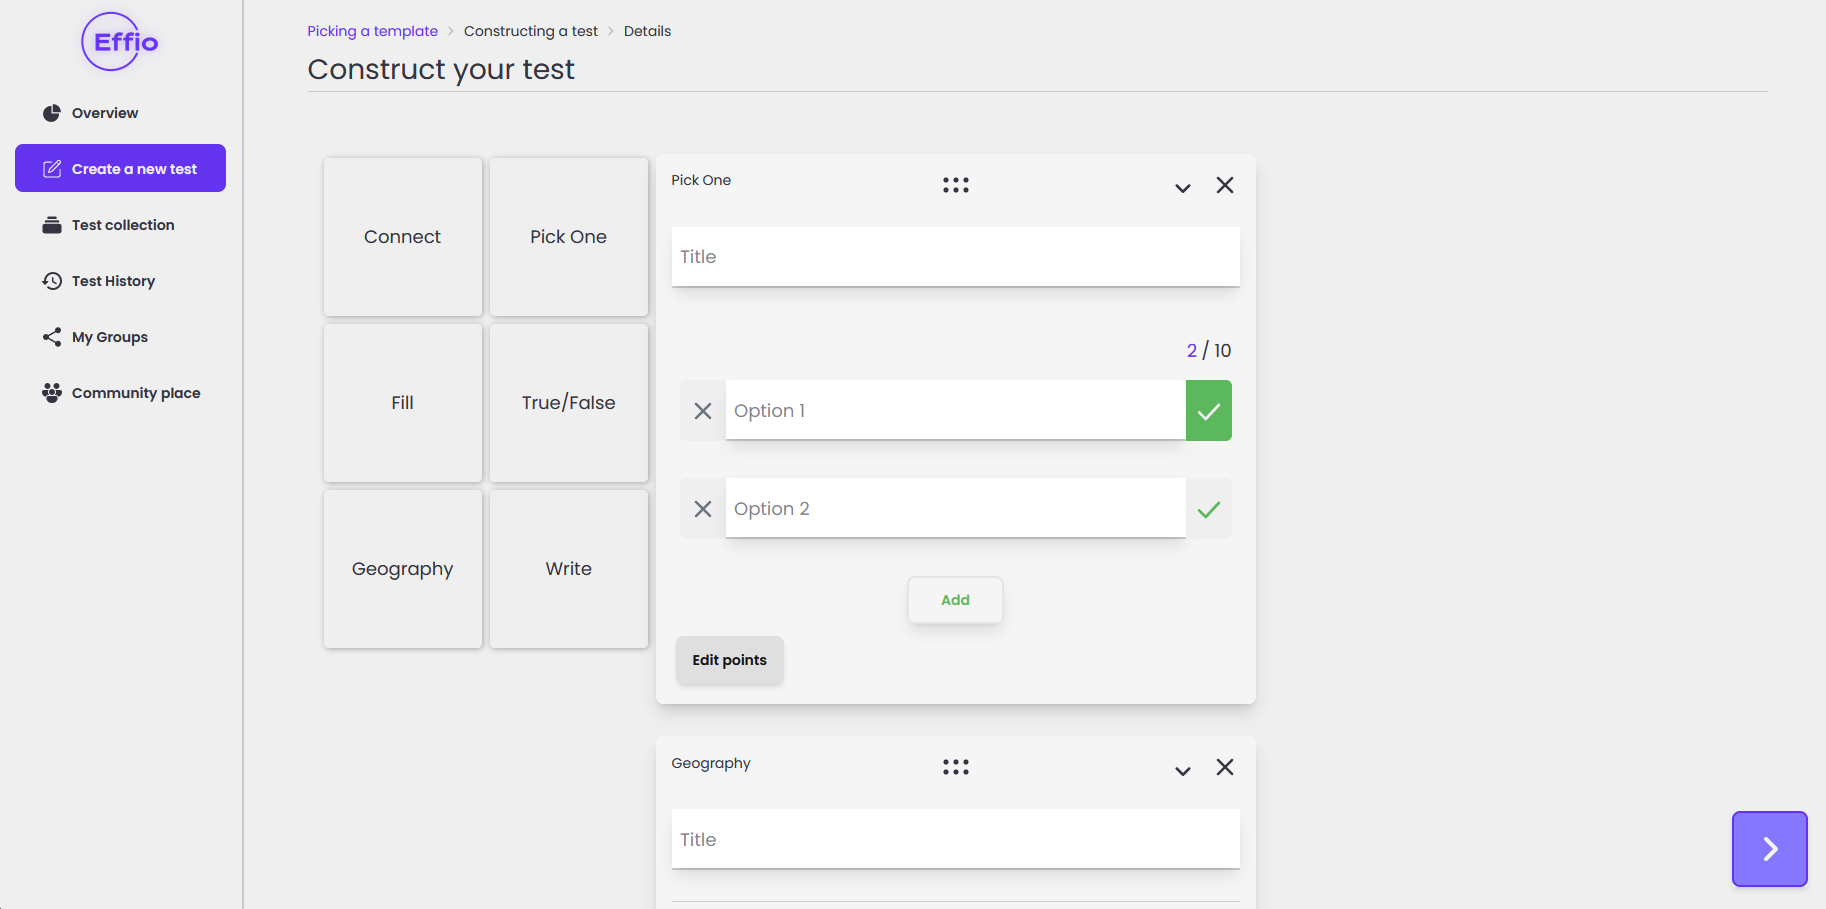
\includegraphics[width=\textwidth]{image/test-creator1.png}
		\caption{Kvízový test}
		\label{fig:test-creator1}
	\end{minipage}
	\hfill
	\begin{minipage}[]{0.49\textwidth}
		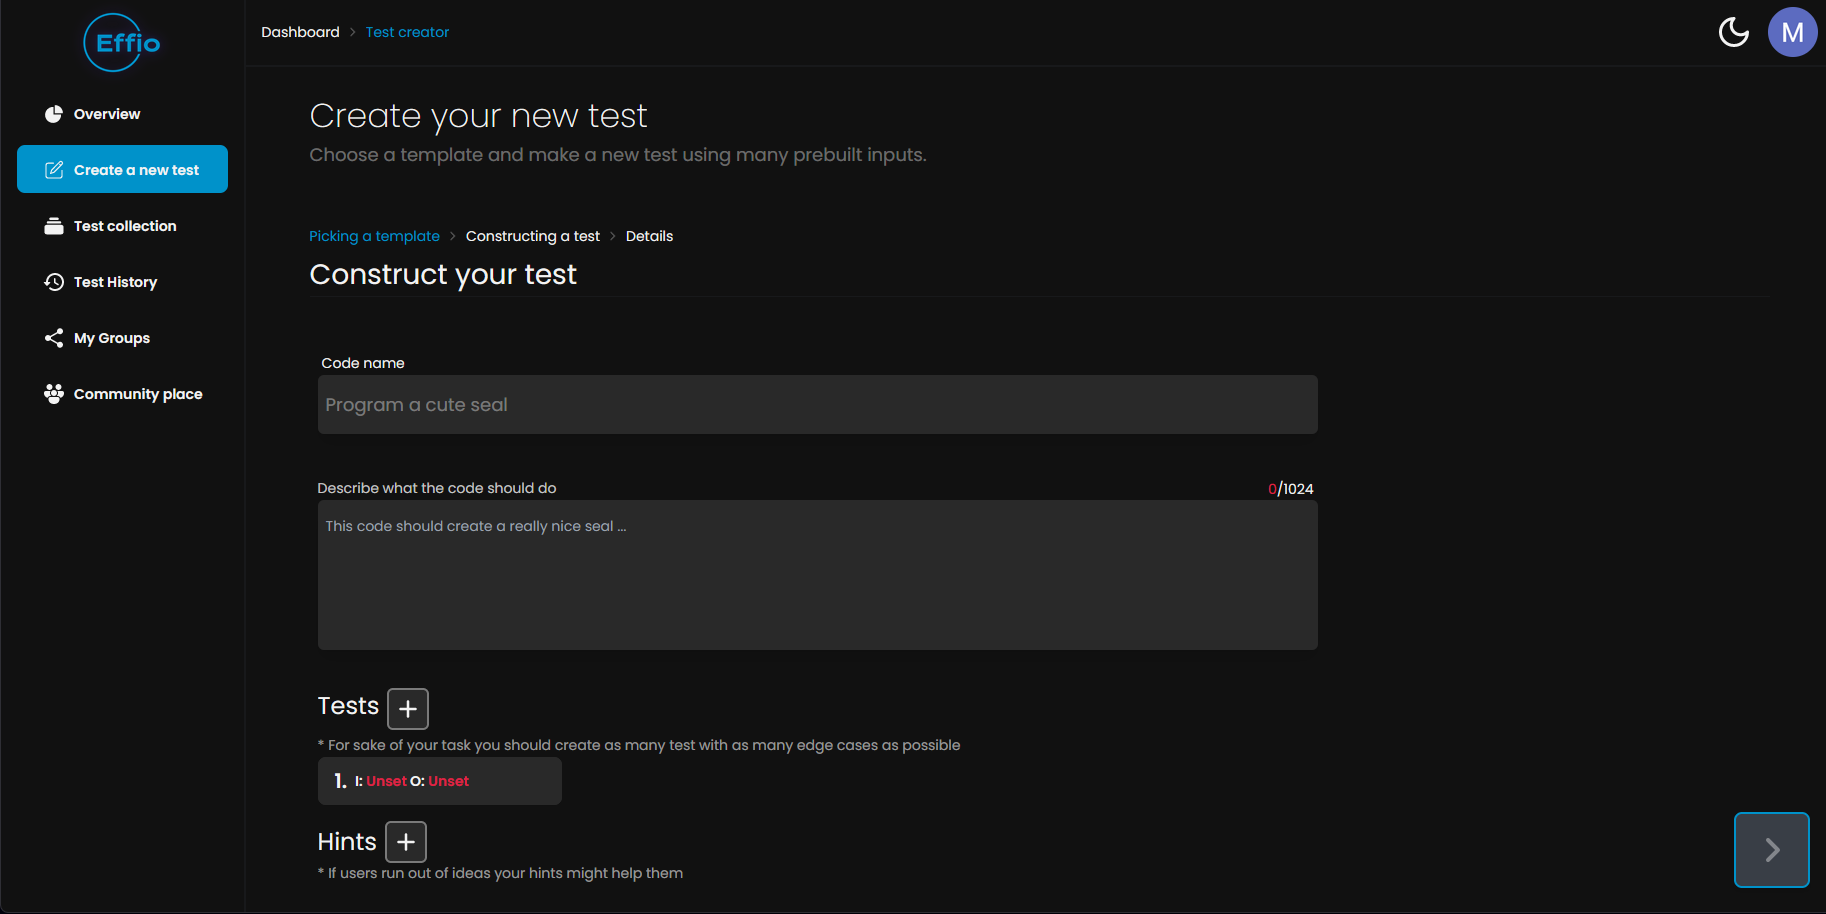
\includegraphics[width=\textwidth]{image/test-creator2.png}
		\caption{Programovací test}
		\label{fig:test-creator2}
	\end{minipage}
\end{figure}

\section{Vyplňování testu}
\label{sec:test-take}
\subsection{Vyplňování kvízu}
Vytvořený test si poté může kdokoliv s~přístupem k~němu vyplnit (testy jsou základně dostupné pro všechny, po úpravě mohou být zveřejněny pouze pro členy skupin).

Otázky se náhodně seřadí a uživatel je vyplňuje, zamíchané jsou také odpovědi určitých typů otázek. Po vyplnění všech uživatel test odevzdá, zkontroluje se a vrátí mu správné odpovědi, počet bodů, známku co získal a pokud je uživatel přihlášený tak se záznam a vyplnění uloží do databáze, uživatel si ho poté může zpětně zobrazit v sekci \textit{Test history}.

\begin{figure}[H]
	\centering %% příkaz, který ti obrázek zarovná na střed
	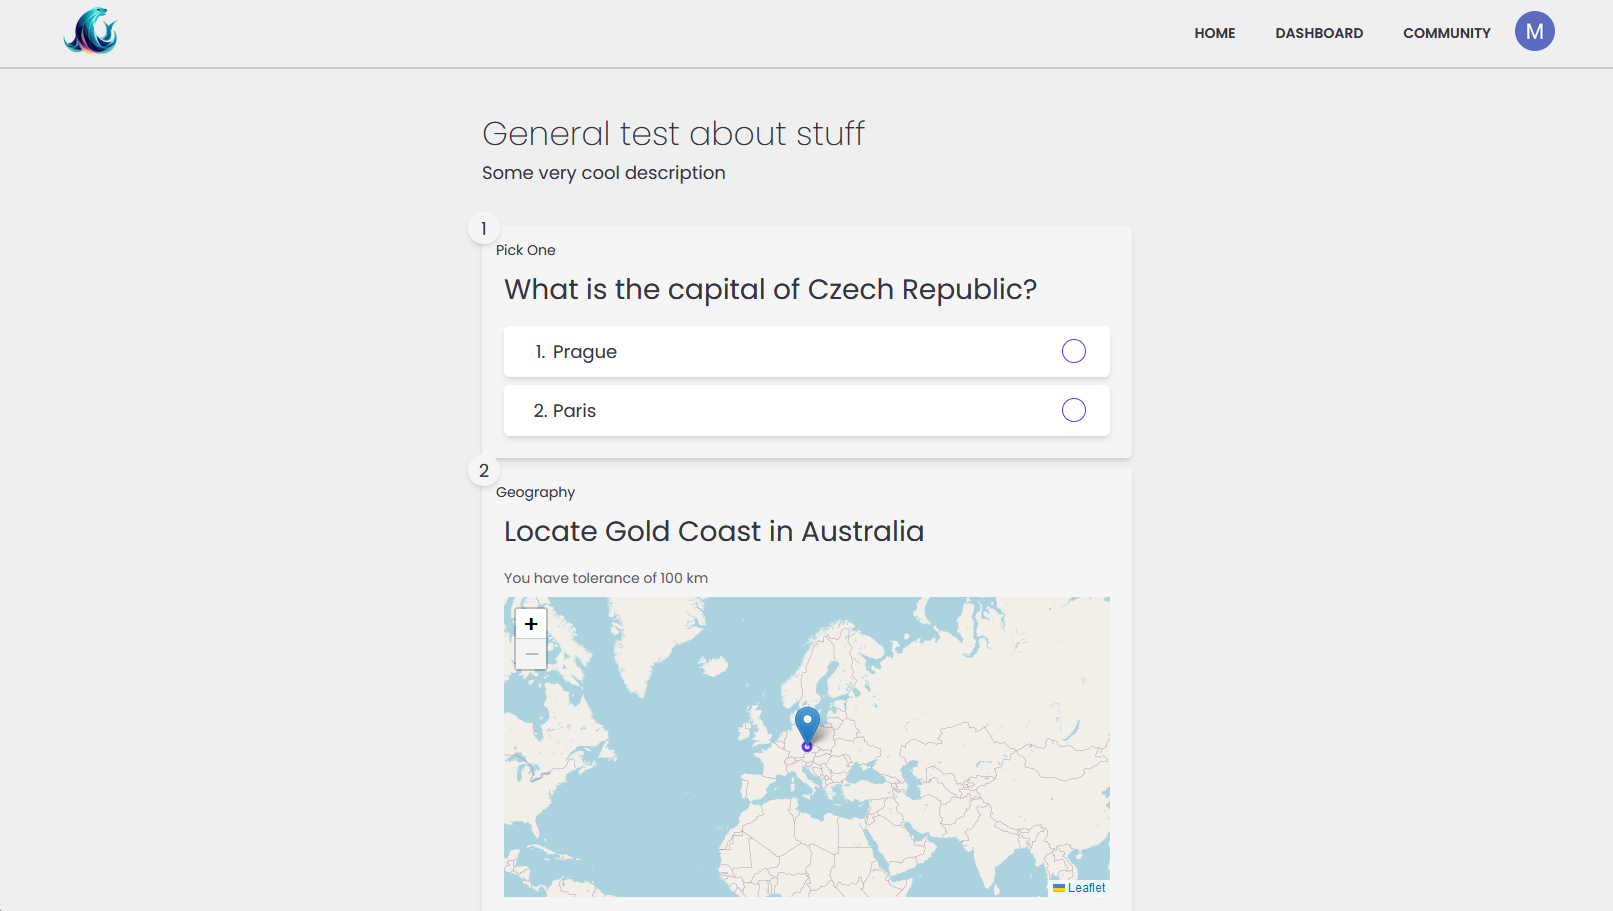
\includegraphics[width=0.75\linewidth]{image/test-taking.png} 
	\caption{Obrázek kvízu.} %% popisek obrázku, nezapomeň na citace!
	\label{fig:test-taking} %% označení až budeš chtít na obrázek odkazovat
\end{figure}

\subsection{Plnění programovacího testu}
Uživatel dostane popis toho co by měl kód umět, sadu testů, které mají otestovat funkcionalitu kódu a popřípadě nějaké nápovědy. Programovací test obsahuje vlastní editor do kterého uživatel píše, pro kontrolu testu můžeme použít tlačítko \textit{\uv{Run}} a pokud testy prochází tak je test možné řešení odevzdat.

\begin{figure}[H]
	\centering %% příkaz, který ti obrázek zarovná na střed
	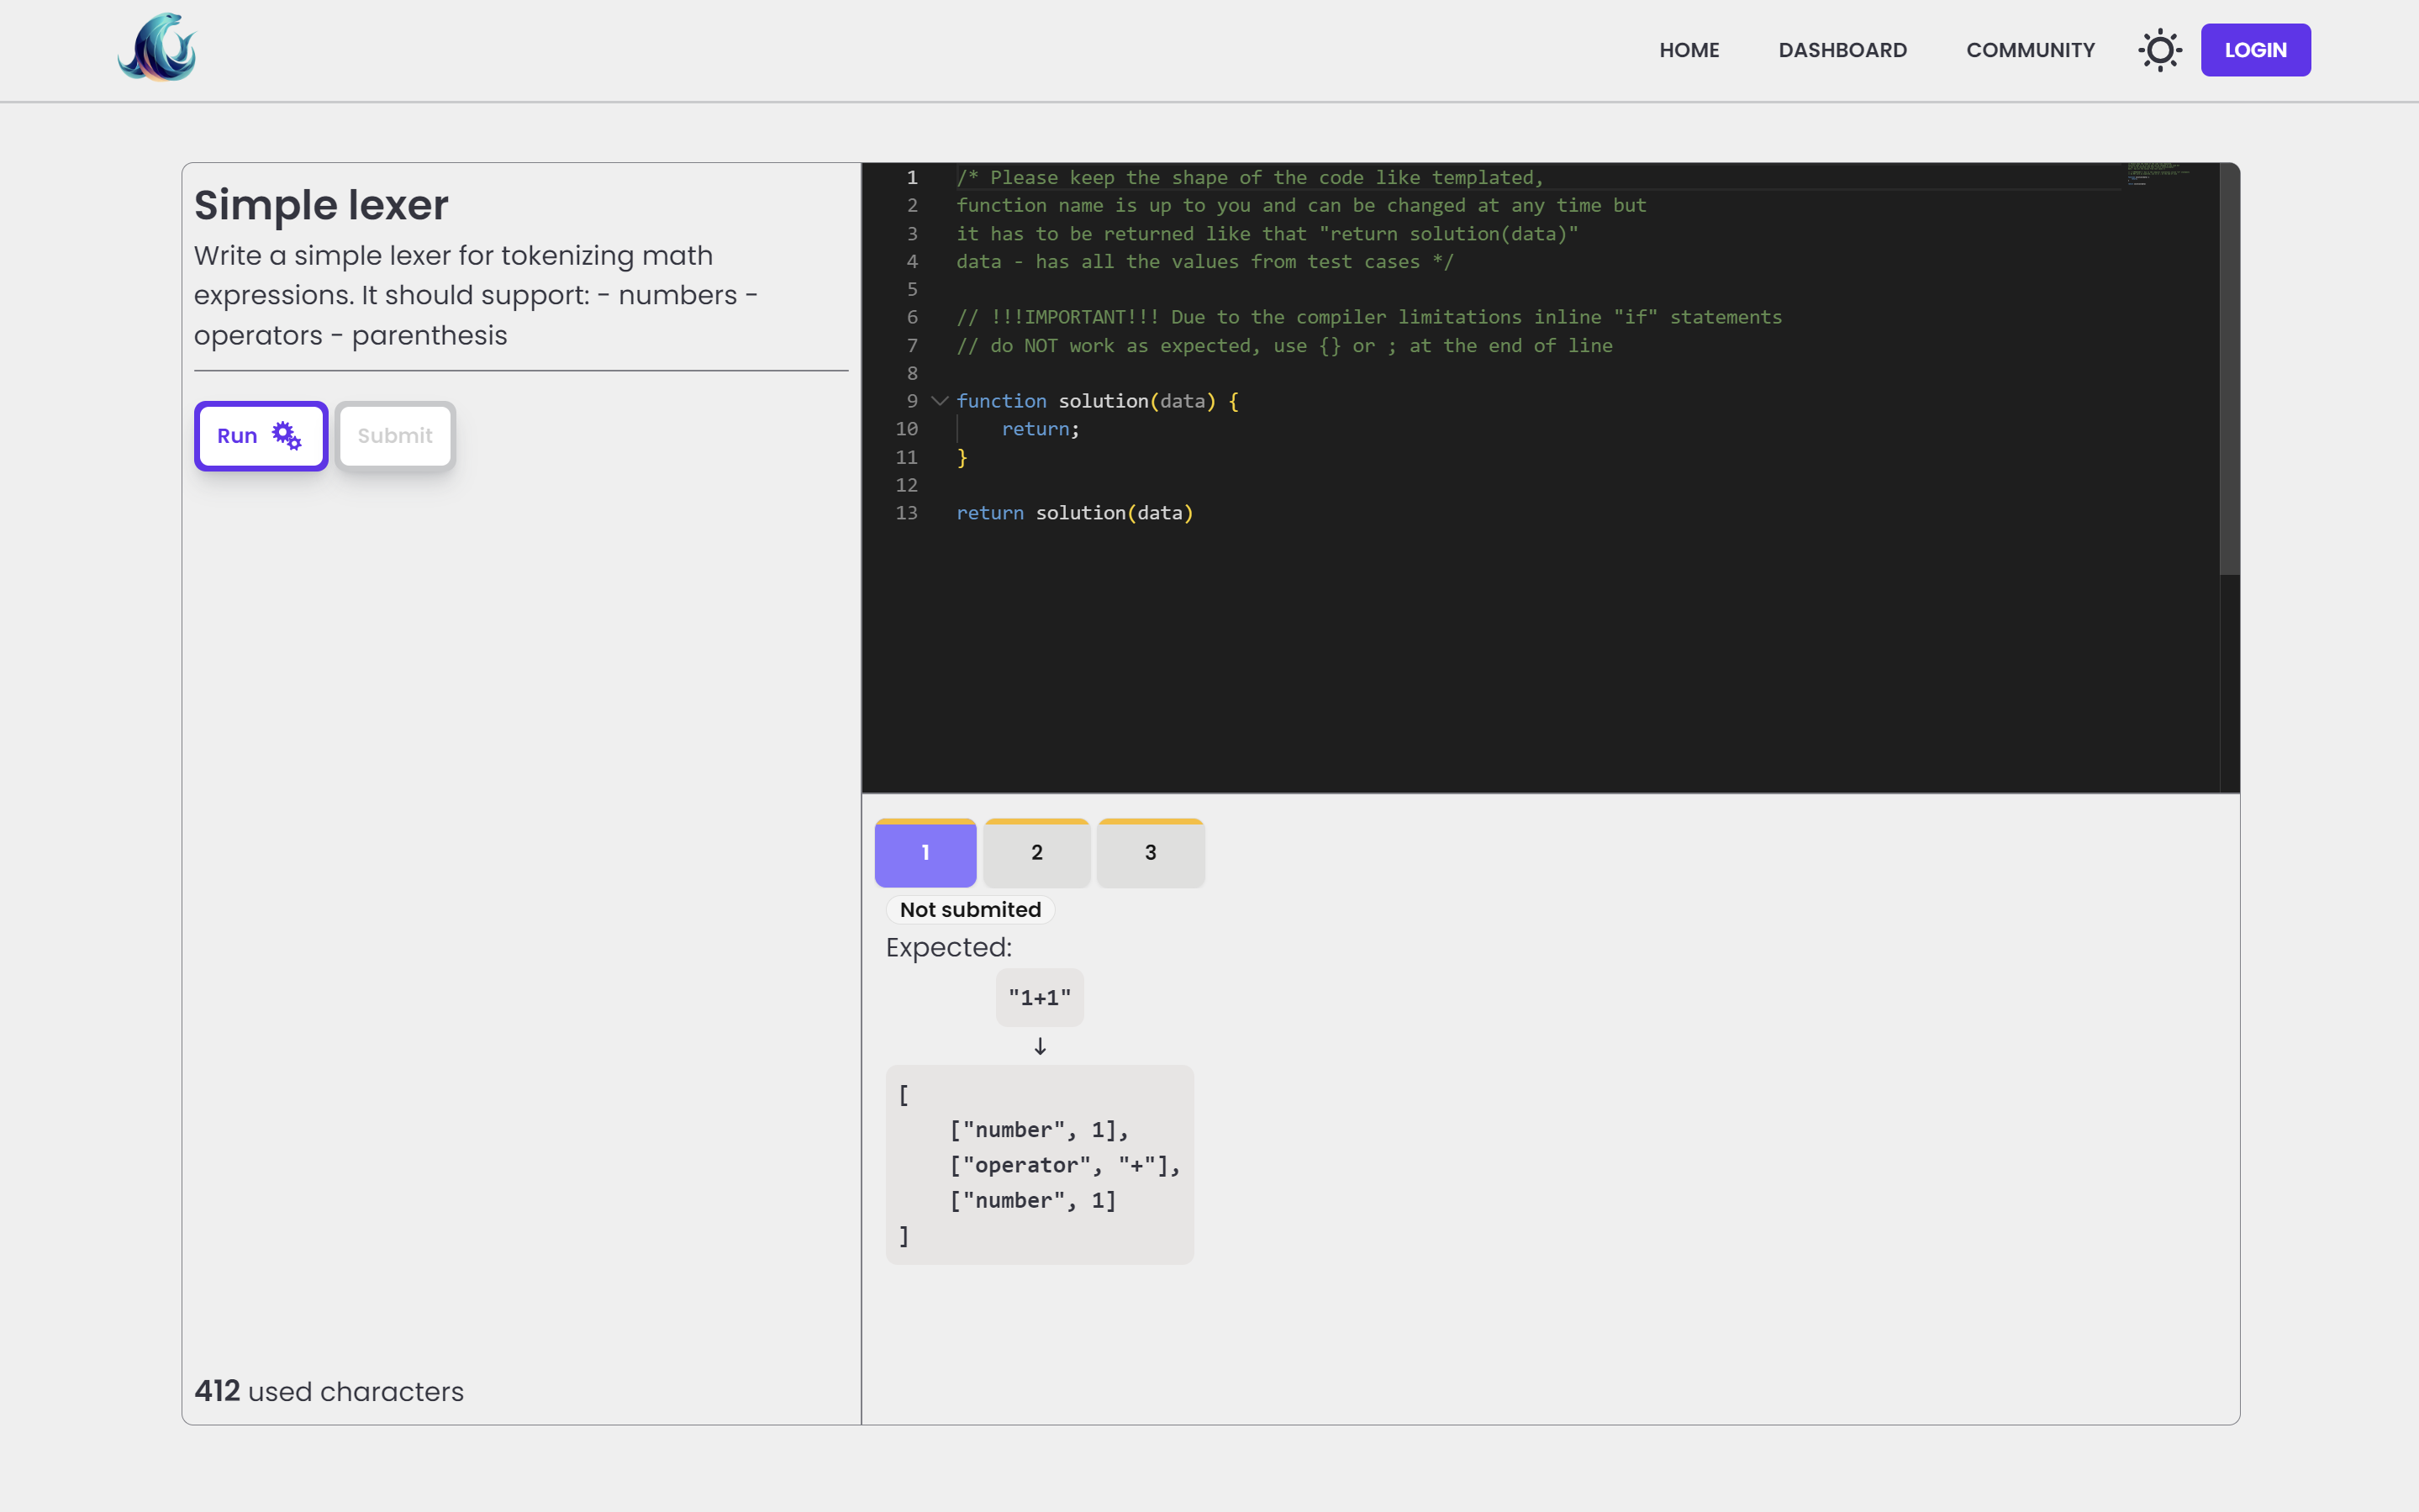
\includegraphics[width=0.75\linewidth]{image/programming.png} 
	\caption{Obrázek programovací úlohy.} %% popisek obrázku, nezapomeň na citace!
	\label{fig:programming} %% označení až budeš chtít na obrázek odkazovat
\end{figure}


\section{Zobrazování testů}

\subsection{Komunitní místo}
\label{subsec:community}
Na této stránce může uživatel najít nové a populární testy včetně všech testů, které existují. Testy jsou zobrazovány postupně podle techniky \uv{infinite scrolling}, na což využívám JavaScript API Intersection Observer, abych zjistil, kdy uživatel dosáhl posledního prvku a vyžádal si tak další testy. Implementované je vyhledávací pole, které filtruje zobrazované testy, další možností je filtrace pomocí tagů. Vizuálně jsou také rozlišeny kvízy od programovacích testů. Testy se dají ohodnotit hvězdičkou, jejich aplikování využívá principu \uv{optimistic update}, to znamená, že po přidání hvězdičky ji uživatel okamžitě vidí přidanou, zatímco se ověřuje jeho oprávnění a vytváří záznam hvězdičky v databázi. V~případě neúspěchu se poté uživateli sama hvězdička opět odebere. 

\begin{figure}[H]
	\centering %% příkaz, který ti obrázek zarovná na střed
	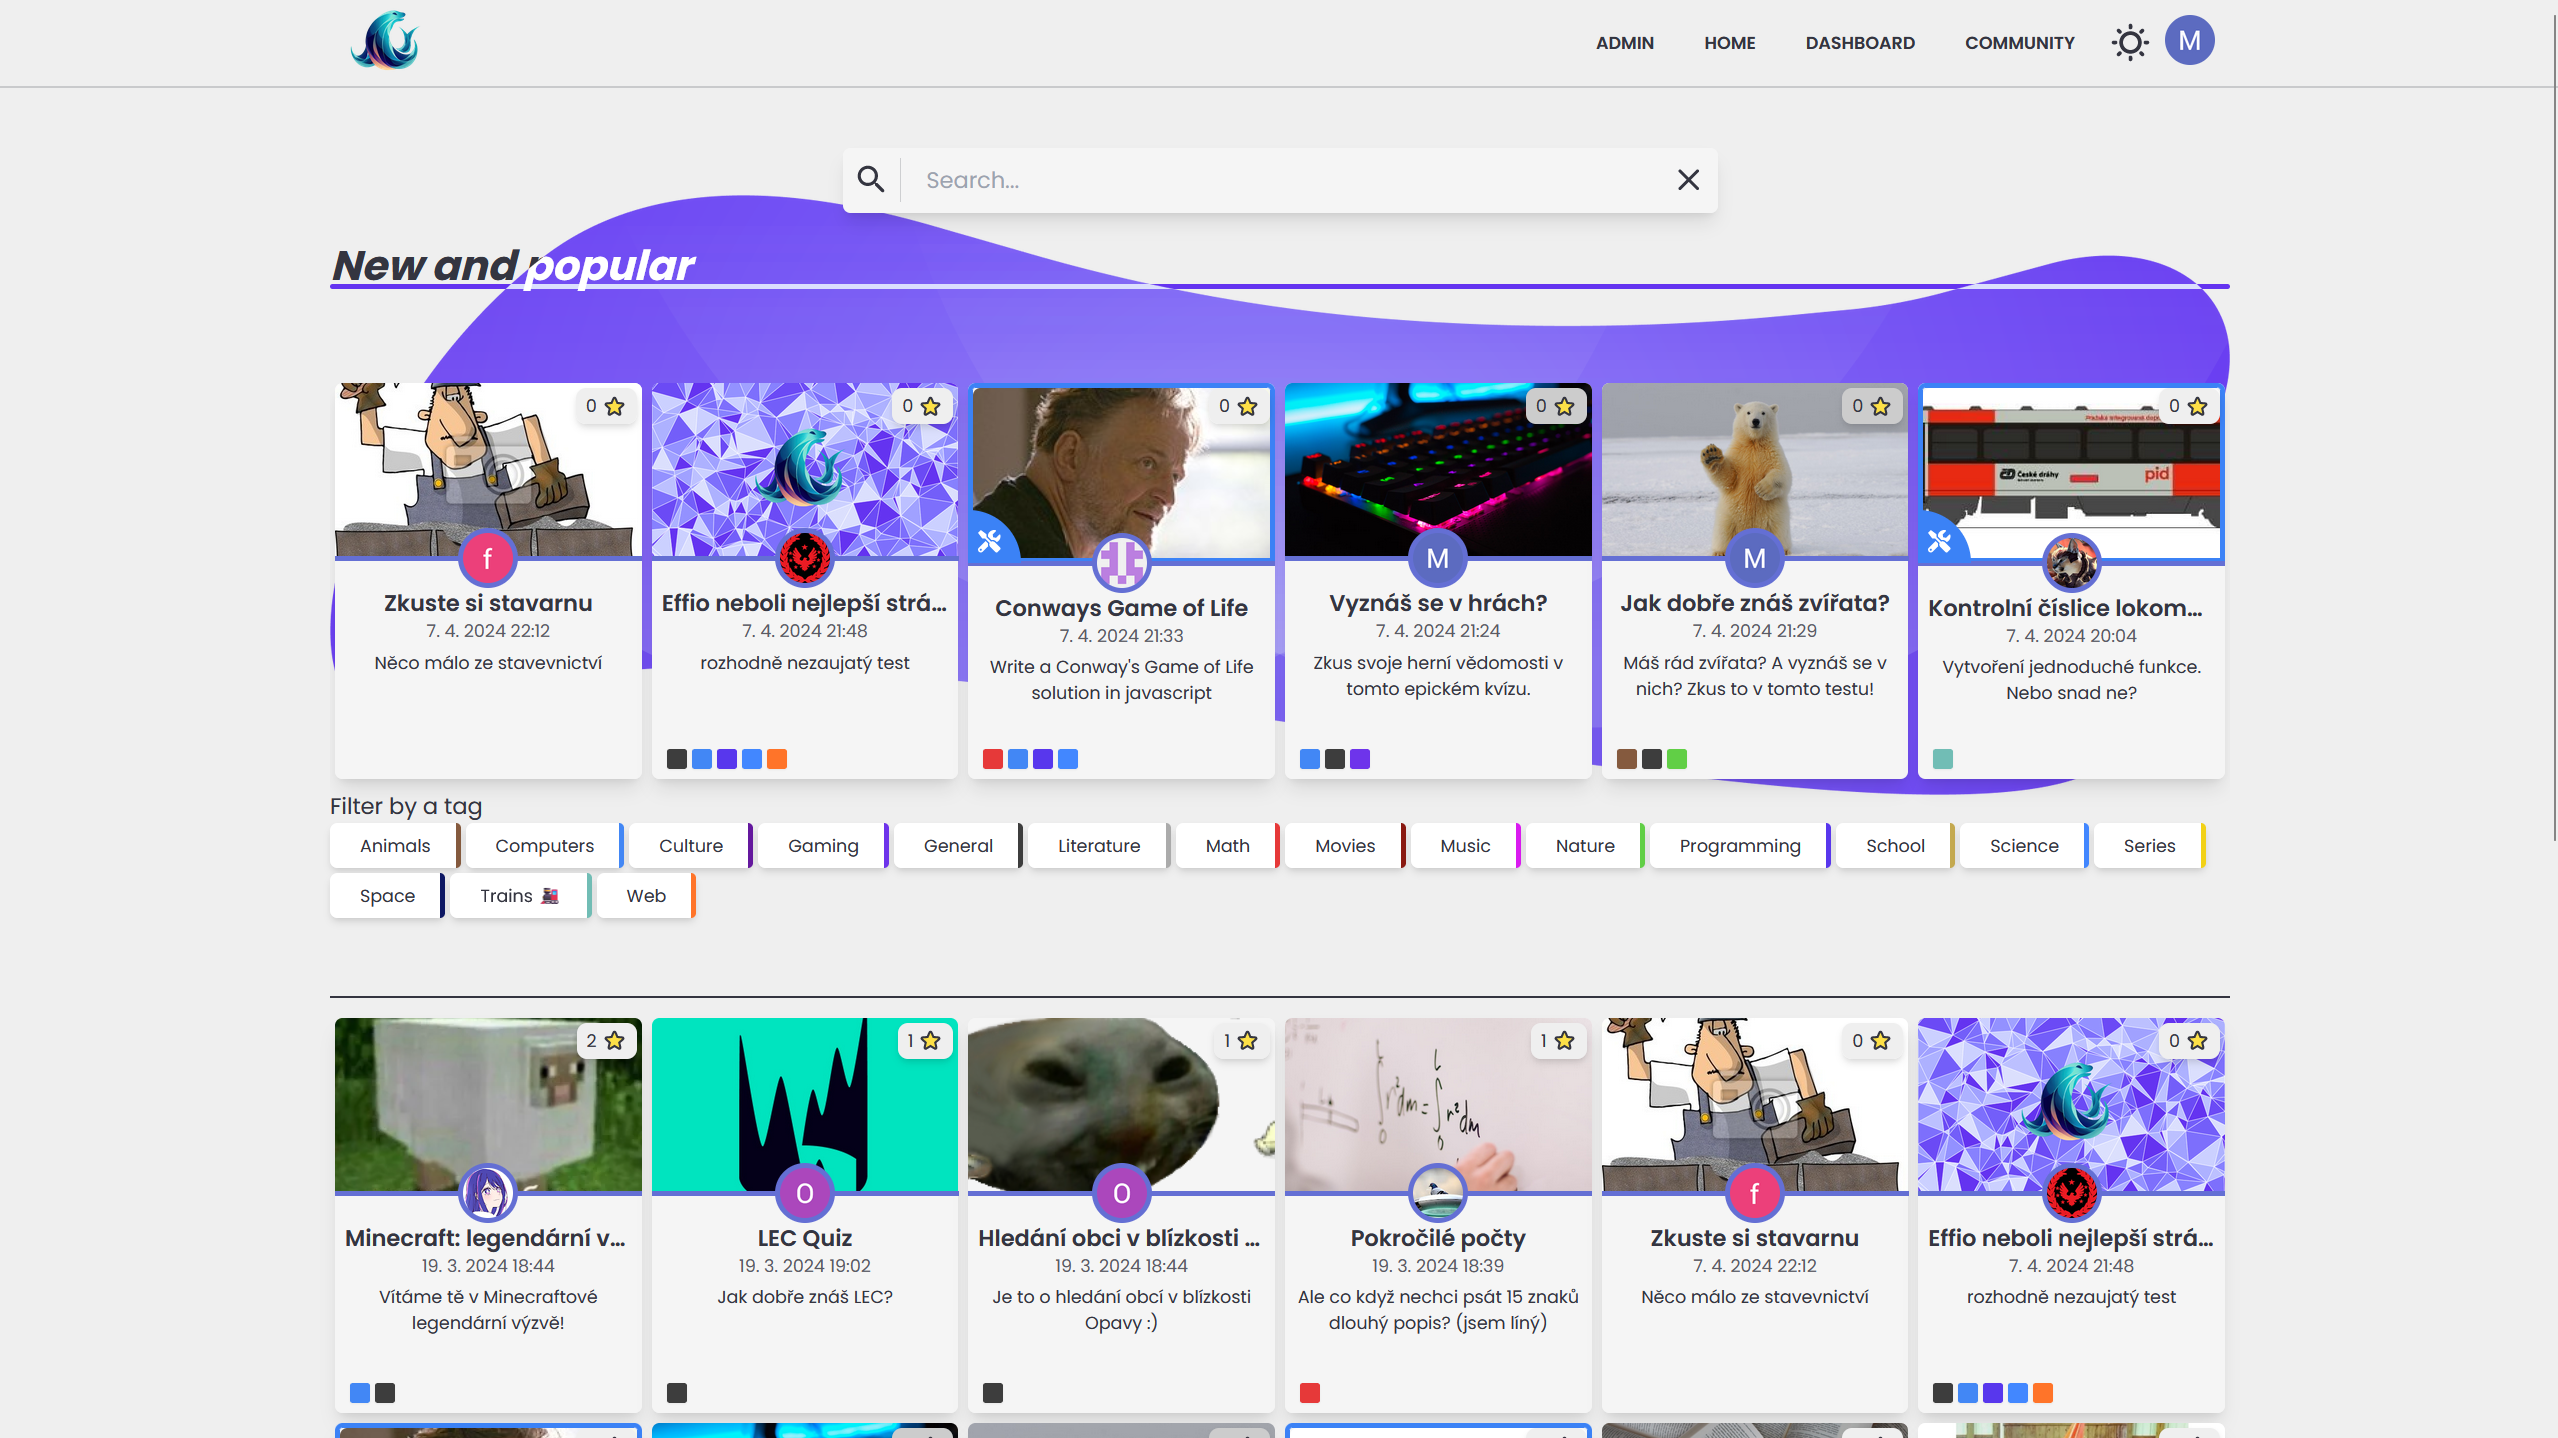
\includegraphics[width=1\linewidth]{image/community.png} 
	\caption{Komunitní místo.} %% popisek obrázku, nezapomeň na citace!
	\label{fig:community} %% označení až budeš chtít na obrázek odkazovat
\end{figure}


\subsection{Kolekce testů}
\label{subsec:collection}
Zde si uživatel může zobrazit jím vytvořené testy, aplikovaná je stejná funkcionalita vyhledávacího pole a \uv{infinite scrollingu}. Každý test má ale také další možnosti, a to úpravu, export a smazání.
\begin{itemize}
	\item Úprava - uživatel se přesune na stránku úprav, tam může celý test přepracovat.
	\item Export - vytvoří z~testu textový soubor ve formátu GIFT se všemi otázkami daného testu, které jsou podporovány Moodlem
	\item Delete - smazání testu z databáze
\end{itemize}


\section{Skupiny}
Každý přihlášený uživatel si může vytvořit vlastní skupinu, do které se můžou pomocí generovaného kódu připojit ostatní uživatelé. Skupina obsahuje kanály, ve kterých je možné psát textové zprávy, taky zde můžeme nají přidané testy, vlastník si poté může procházet grafy výsledku členů skupiny.


\section{Světlý a tmavý režim}
S ohledem na uživatele co preferují tmavý režim jsem se také rozhodl pro tvorbu tmavého režimu, ten je možné vidět na obrázku \ref{fig:test-creator2}, oba tyto režimy vyžadovali vlastní paletu barev a byly mnohokrát přepracovány aby k~sobě jednotlivé barvy co nejlépe pasovaly.

\section{Domovská stránka}
Domovská stránka slouží jako místo pro seznámení návštěvníka s~výhodami Effia, rychlá navigace mezi jednotlivými stránkami ale také jako místo nejpečlivěji vytvářeného designu a efektů aby na uživateli zanechala dojem kvalitní aplikace.

\begin{figure}[h]
	\centering %% příkaz, který ti obrázek zarovná na střed
	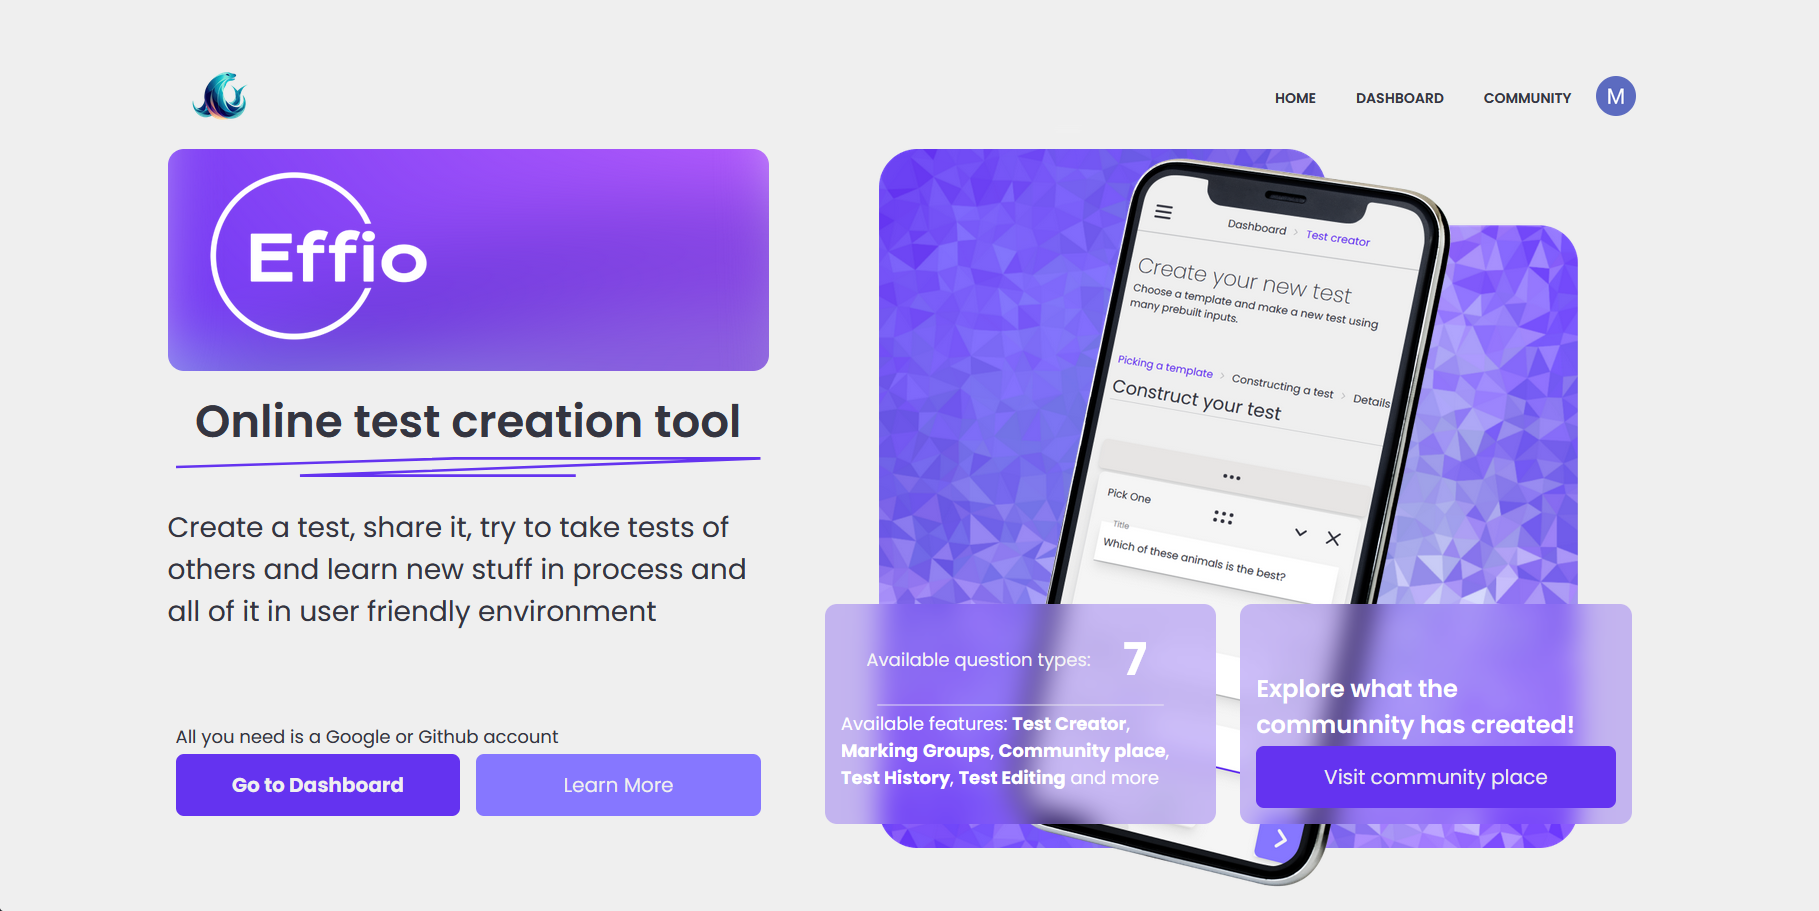
\includegraphics[width=1\linewidth]{image/homepage.png} 
	\caption{Domovská stránka Effia.} %% popisek obrázku, nezapomeň na citace!
	\label{fig:homepage} %% označení až budeš chtít na obrázek odkazovat
\end{figure}
\clearpage
\section{Responsivita}
Celá aplikace je uzpůsobená jak pro počítače tak pro mobilní zařízení. Responsivita není vůbec lehká práce, mně ale pomohl Tailwind, ve kterém se CSS media query dělají snadněji společně s moderními CSS containers, které umožňují responsivní breakpointy odvozovat ne jen od velikosti stránky ale od rozměrů rodičovských elementů.

\begin{figure}[h]
	\centering
	\begin{minipage}[]{0.49\textwidth}
		\centering
		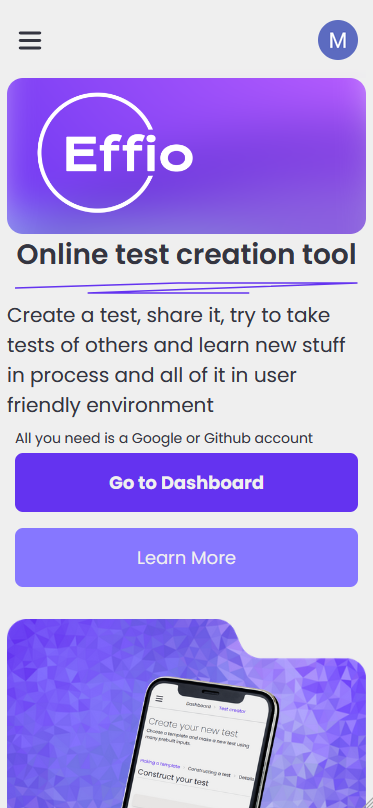
\includegraphics[width=0.5\linewidth]{image/res1.png}
		\caption{Domovská stránka na mobilním zařízení}
		\label{fig:res1}
	\end{minipage}
	\hfill
	\begin{minipage}[]{0.49\textwidth}
		\centering
		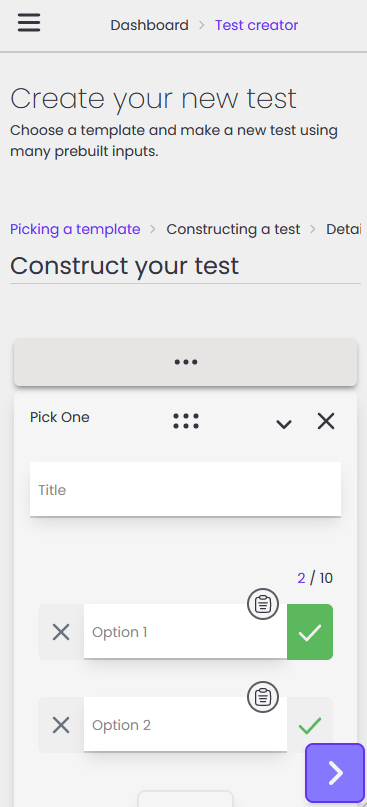
\includegraphics[width=0.5\linewidth]{image/res2.png}
		\caption{Generátor testů na mobilním zařízení}
		\label{fig:res2}
	\end{minipage}
\end{figure}

\chapter{Výsledky práce}
\section{Funkce aplikace}
Po příchodu na stránku se uživateli zobrazí domovská stránka, zde může prozkoumat výhody aplikace nebo se přihlásit, to ho přesune na přihlašovací stránku, na ni se uživatel do aplikace může přihlásit pomocí Google nebo GitHub účtu. Po přihlášení je uživatel přesunut na dashboard, kde může vidět rychlou navigaci na další části nebo se podívat na souhrn jeho aktivity v~grafech. První možností je vytvořit si nový test, tato možnost je detailně probraná zde \ref{subsec:creation}.
Po vytvoření testu je přesunut do kolekce jeho testů, kde může své testy procházet a upravovat, více popsáno zde \ref{subsec:collection}. Test si poté může uživatel zkusit vyplnit \ref{sec:test-take}, buď přímo ze své kolekce nebo z komunitního centra \ref{subsec:community}, kde může najít také testy jiných. Po dokončení testu se dozví výsledky, ty může poté najít zpětně v~sekci \textit{Test history}, kde jsou uspořádané v tabulce.

\section{Splněné a nesplněné cíle}
Cíle byly rozdělené jak do rozsahu aplikace tak do kvality implementace jednotlivých prvků, co se týče rozsahu tak ten jsem v~určitých místech významně předčil, ne všechny body původních cílů jsou ale aktuálně plně dosaženy.

Hlavním cílem bylo vytvořit rychlou, cloudovou aplikaci pro vytváření a sdílení testů využívající moderních \uv{techstack}, v~tomto ohledu jsem cíl kompletně splnil, aplikace je v~těchto bodech plně funkční a můj původní plán využití technologií se během vývoje ještě významně rozrostl.

Za úspěch považuji také grafickou část aplikace, která za mě tvoří minimalistický moderní vzhled.

Hlavní neúspěch nebo spíše nedodělanost vidím ve skupinách a přizpůsobení možností testů pro ně, původně jsem zamýšlel vytvořit skupiny jako místo pro sdílení materiálů s více zajímavými možnostmi pro vlastníka, aby sloužili jako funkce vhodná pro výuku. Cíle nejsou zdaleka nerealistické, ale těchto cílů jsem nebyl schopen dosáhnou z~nedostatku času, jako vylepšení by ale za mně bylo velice přínosné.
	
\chapter*{Závěr}
	
Cílem projektu bylo vytvořit webovou aplikaci pro vytváření a vyplňování testů. Aplikace je postavená na frameworku SvelteKit, psaný v jazyce TypeScript. Přihlašování stojí na knihovně Auth.js, MySQL databáze je hostovaná službou Planetscale, jako ORM je použita Prisma. Frontend řeší framework Svelte s~CSS utility knihovnou Tailwind, pro validaci využívá Zod.

Základem aplikace je generátor testů, kde uživatel využívá předpřipravené typy otázek. Testy se následně dají vyplnit v rámci komunity nebo vlastníkovi kolekce. Nepřihlášený uživatel může testy pouze vyplňovat, přihlásit se uživatel může pomocí Google nebo GitHub účtu. Uživatelé také mají k~dispozici skupiny kde je chat a také možnosti sdílet testy, test historii k~zobrazení dříve vyplněných testů a přehled nedávné aktivity v podobě grafů. Využité technologie činí aplikaci lehce škálovatelnou a velice výkonnou. Aplikace je téměř zcela funkční a použitelná na všech zařízeních díky responzivnímu designu.

\noindent Aplikace je zálohovaná na GitHubu na adrese \url{https://github.com/matej-kotrba/effio}.
Je také volně přístupná na adrese \url{https://effio.vercel.app/}
	
	%% literatura
	\begin{thebibliography}{99}
		
		\bibitem{Svelte} Svelte [online]. 2023 [cit. 2023-12-27]. Dostupné z: \url{https://svelte.dev/}
		\bibitem{SvelteKit} SvelteKit [online]. 2023 [cit. 2023-12-27]. Dostupné z:  \url{https://kit.svelte.dev/}
		\bibitem{tRPC} tRPC [online]. 2023 [cit. 2023-12-27]. Dostupné z: \url{https://trpc.io/}
		\bibitem{Prisma} Prisma [online]. 2023 [cit. 2023-12-27]. Dostupné z: \url{https://www.prisma.io/}
		\bibitem{Zod} Zod [online]. 2023 [cit. 2023-12-27]. Dostupné z: \url{https://zod.dev/}
		\bibitem{Auth.js} Auth.js [online]. 2023 [cit. 2023-12-27]. Dostupné z: \url{https://authjs.dev/}
		\bibitem{Tailwind CSS} Tailwind CSS [online]. 2023 [cit. 2023-12-27]. Dostupné z: \url{https://tailwindcss.com/}
		\bibitem{tRPC-SvelteKit} tRPC-SvelteKit [online]. 2023 [cit. 2023-12-27]. Dostupné z: \url{https://icflorescu.github.io/trpc-sveltekit/}
		\bibitem{ChatGPT} ChatGPT [online]. 2023 [cit. 2023-12-27]. Dostupné z: \url{https://chat.openai.com/}
		\bibitem{Stackoverflow} Stackoverflow [online]. 2023 [cit. 2023-12-27]. Dostupné z: \url{https://stackoverflow.com/}
		\bibitem{Joy of Code}Joy of Code. Youtube kanál. Https://www.youtube.com/ [online]. 2023 [cit. 2023-12-27]. Dostupné z: \url{https://www.youtube.com/@JoyofCodeDev}
		\bibitem{Huntabyte}Huntabyte. Youtube kanál. Https://www.youtube.com/ [online]. 2023 [cit. 2023-12-27]. Dostupné z: \url{https://www.youtube.com/@Huntabyte}
		\bibitem{Theo}BROWNE, Theo. Youtube kanál. Https://www.youtube.com/ [online]. 2023 [cit. 2023-12-27]. Dostupné z: \url{https://www.youtube.com/@t3dotgg}
		\bibitem{Kevin Powell}POWELL, Kevin. Youtube kanál. Https://www.youtube.com/ [online]. 2023 [cit. 2023-12-27]. Dostupné z: \url{https://www.youtube.com/@KevinPowell}
		\
		
	\end{thebibliography}
	
	%% obrázky 
	\listoffigures
	

	\appendix %% začínají přílohy
	
	\titleformat{\chapter}[block]{\scshape\bfseries\LARGE}{Příloha \thechapter}{10pt}{\vspace{0pt}}[\vspace{-22pt}] %% nastavení nadpisu u příloh
	

	
\end{document}